
\documentclass[10pt, a4paper, twoside]{article}
\usepackage[utf8]{inputenc}
\usepackage{authblk}
\usepackage{multicol}
\usepackage{abstract}
\usepackage{xcolor}
\usepackage[a4paper, total={6in, 8in}]{geometry}
\usepackage{biblatex}
\usepackage{graphicx}
\usepackage{newfloat}
\usepackage{hyperref}
\DeclareFloatingEnvironment[name={Supplementary Figure},fileext=lsf,listname={List of Supplementary Figures}]{suppfigure}


\setlength{\columnsep}{1cm}
\addbibresource{su2020_cov2.bib}

\graphicspath{{../Figures/}}


\title{Impact of travel-associated cases on the SARS-CoV-2 epidemic in Switzerland from June to September 2020}

\author[1]{Martina L. Reichmuth}
\author[1]{Emma B. Hodcroft}
\author[1]{Julien Riou}
%\author[2,3]{Niel Hens}
\author[1*]{Christian L. Althaus}

\renewcommand*{\Affilfont}{\normalsize\normalfont}
\affil[1]{Institute of Social and Preventive Medicine, University of Bern, Bern, Switzerland}
%\affil[2]{Interuniversity Institute for Biostatistics and statistical Bioinformatics, Data Science Institute, Hasselt University, Hasselt, Belgium}
%\affil[3]{Centre for Health Economics Research and Modelling Infectious Diseases, Vaccine and Infectious Disease Institute, University of Antwerp, Antwerp, Belgium}
\affil[*]{Correspondence: christian.althaus@ispm.unibe.ch}

\renewcommand{\abstractnamefont}{\normalfont\bfseries}
\renewcommand{\abstracttextfont}{\normalfont\small} 


\date{}
\pagenumbering{arabic}
\begin{document}

\maketitle
\begin{abstract}
\noindent 

Introduction: In Switzerland, the severe acute respiratory syndrome coronavirus 2 (SARS-CoV-2) epidemic grew from a few dozen confirmed cases to several hundred cases per day during summer 2020. 
Switzerland and other European countries opened borders to allow for holiday travel. 
The impact of travel-associated cases (imports) on the national epidemic dynamics remains unclear. 
Our objective was to assess the impact of imports on the epidemic from June to September 2020.

Method: We fitted a negative binomial generalised linear model to the daily number of confirmed cases reported by the Federal Office of Public Health (FOPH) to estimate the epidemic growth rate. 
We then used a stochastic branching process model that can account for individual variation in transmission of SARS-CoV-2 to simulate epidemic trajectories using different values for the effective reproduction number $R_e$ (0.6-1.2) and number of imports (3,304-14,582).

Results: From June to September 2020, 23,199 SARS-CoV-2 cases were reported. 
For 12,259 (52,84\%) cases the likely place of infection was reported, i.e. for 8,955 a national and 3,304 an international infection place was stated. 
In absence of imports, we estimated an epidemic growth rate of 0.023 (95\% confidence interval (CI): 0.021-0.024) per day. 
We found that increasing the number of imports requires lower values of $R_e$ to account for the dynamic. 
For example, 3,304 imports (as reported) would have been sufficient to account for the observed epidemic dynamics despite $R_e < 1$, i.e., a value below the critical threshold.

Discussion: Quantifying the role of imports on the national dynamics of SARS-CoV-2 epidemics requires further investigation. 
In Switzerland, imported cases might have had a considerable impact on the national dynamics and can explain the growth of the SARS-CoV-2 epidemic during summer 2020. 
Our results underline the importance of improved surveillance for international travellers in order to better control the spread of SARS-CoV-2.
\clearpage
\end{abstract}


\begin{multicols}{2}
\section{Introduction}
In spring 2020, travel-associated cases of the severe acute respiratory syndrome coronavirus 2 (SARS-CoV-2) were likely to have caused a high proportion of cases in many countries.\cite{russell_effect_2021} 
In the absence of travel restrictions, countries can expect travel-associated cases.\cite{russell_effect_2021} 
Travel restrictions might contribute to epidemic control in many countries, whereas in others, travel-associated cases are likely to contribute little to local SARS-CoV-2 epidemics.\cite{russell_effect_2021}  
Russell et al., 2021 recommended that authorities evaluate the effect of travel-associated cases on the local SARS-CoV-2 incidence, local epidemic growth, and travel volumes before implementing such restrictions.\cite{russell_effect_2021} 
During summer 2020, Switzerland and other European countries had reopened borders to allow for travel. 
In Switzerland borders were reopened on the $15^{th}$ of June 2020 to \textcolor{red}{most/all (European)} countries. 
Due to Switzerlands prominent location in the heart of Europe - with boarders to Germany, France, Italy, Austria, and Principality of Liechtenstein - , many different countries are easily visited and vis-versa many citizens from different countries might visit Switzerland. 
Phylogenetic analysis showed that SARS-CoV-2 strains that most likely originated in Spain spread to several other countries including Switzerland.\cite{hodcroft_emergence_2020}
In summer 2020, Switzerland had a population of 8,5 millions and the SARS-CoV-2 epidemic grew from a few dozen confirmed cases per day in early June 2020 to several hundred cases per day by the end of September 2020. 


The dynamic of an epidemic can be explained with the effective reproduction number $R_e$. 
$R_e$ is the average number of secondary cases per infectious case in the population of both susceptible and non-susceptible individuals. 
Where $R_e > 1$ , the number of cases will increase, where $R_e = 1$, the disease is endemic, and where $R_e < 1$ there will be a decline in the number of cases. 
For airborne diseases such as SARS-CoV-2 the individual variation in transmission is difficult to measure empirically. 
Lloyd-Smith et al., 2005 showed that the population dynamic can be explained with mathematical models that allow for individual variation.\cite{lloyd-smith_superspreading_2005}  
Thus, secondary cases might be described with a negative binomial distribution. Depending on the dispersion parameter $k$ the probability of stochastic extinction and outbreaks varies widely. 
Disease control interventions could influence the individual variation in infectiousness.\cite{lloyd-smith_superspreading_2005} 
Lloyd-Smith et al., 2005 showed that outbreaks are rarer but more explosive and extinction is more likely with a small $k$ then with $k = 1$ that equals the geometric distribution and $k = \infty$ that equals the Poisson distribution.\cite{lloyd-smith_superspreading_2005} 
The later accounts for no individual variation. 
Thus, the extinction probability in a stochastic model varies with $R_e$, $k$ and the number of infections at the start, i.e. seeds. 
The $R_e$ can be estimated by the epidemic growth rate, the generation time resulting in a shape parameter, and rate parameter of the gamma distribution. 
The generation time is an interval from when a susceptible is infected by an infected individual to when this individual was infected. 
These periods of infecting others can be explained using a gamma distribution. 
For SARS-CoV-2, the generation time was estimated to be 5.2 days with a standard deviation (SD) of 2.8.\cite{ganyani_estimating_2020}

The impact of travel-associated cases (in the method and result section called imports) on the Swiss national epidemic dynamics remains unclear.
Our objective was to assess the impact of imports on the SARS-CoV-2 epidemic in Switzerland during summer 2020.

\section{Method}

\subsection{Data availability}
We analysed the epidemic from $1^{st}$ of June to $30^{th}$ of September 2020. 
For the propose of this study, we used confidential data reported by the Federal Office of Public Health (FOPH). 
Data included date of diagnosis, or registration, date of hospitalisation, date of death, and age of individual. 
Moreover, the most likely country of infection might be listed.

\subsection{Definition}
We have listed the 23 most frequently reported places of infection. Other countries were included in 'others'. None of these countries were reported more than ten times.
We analysed the age (in years) and also introduced the following categories: adolescents and young adults (16-30 years), adults and families (31-50 years and children up to 15 years) and older adults ($>$ 50 years) on.


The $R_e$ is given by $(1 + \frac{r}{\beta} )^\alpha$ where $r$ is the epidemic growth rate, $\alpha$ the gamma shape parameter, and $\beta$ is the rate parameter of the gamma distribution. 
The parameter $\alpha$ is given by the generation time $\mu$ (here 5.2 days) and its variance $\sigma^2$ (here 7.8 days) as $\frac{\mu^2}{\sigma^2 }$ and $\beta$ is given as $\frac{\mu}{\sigma^2}$. 
The distribution of secondary cases can be described with a negative binomial distribution with the mean $R_e$ and its variance of $R_e$ as $\frac{R_e}{1+\frac{R_e}{k}}$ where $k$ is the over-dispersion parameter. 
The stochastic probability of extinction was estimated for each $k$, namely 0.1, 0.5, 1, and  $\infty$. 
Extinction was assumed if there were no cases for at least $\mu + 3*\sigma$ days (here 14 days) at the end of the period of interest.
The probability of stochastic extinction then resulted from the number of simulations that met the extinction criteria, divided by all simulations (here $10^3$).

\subsection{Statistics}
We fitted a negative binomial generalised linear model to the daily number of confirmed cases, hospitalised cases, and deaths adjusted for weekends (using the MASS-package).\cite{venables_modern_2002} 
Later, we used these three models and estimated a weighted epidemic growth rate $r$ and the $R_e$ (as described in section 2.2). 
We predicted the epidemic curve for the time of interest ($1^{st}$ of June to $30^{th}$ of September 2020) with a seed of 50 cases on the $31^{st}$ of May. 
Further, we used a stochastic branching process model that can also account for individual variation in transmission of SARS-CoV-2 using a dispersion parameters $k$ of 0.1, 0.5, 1, and  $\infty$ to simulate epidemic trajectories. 
Each scenario was simulated $10^3$ times.
We included seeds for the previous five days, i.e. 27$^{th}$ to 31$^{st}$ May 2020.
These seeds were calculated from the fitted model using the daily number of confirmed cases and multiplied by two.
In the stochastic models, we varied the value of $R_e$ (from 0.6 to 1.2 in 0.1 steps) and the number of imports.
We simulated epidemic trajectories including imports that transmitted further. 
We simulated trajectories for reported imports, reported imports multiplied by $1+ \frac{\Sigma ~of ~cases ~with ~unknown ~origin }{\Sigma ~of ~all ~confirmed ~cases}$. 
The number of imports per day was multiplied with 1, 2, and 3. 
As a sensitivity analysis, we allowed no further transmission for imports. 
All analyses were preformed using $R ~v.1.3.1093$.\cite{r_core_team_r_2020}


\subsection{Ethics}
\textcolor{red}{As we use FPOH data, do we have to state sth?}

\section{Results}
In total 23,199 cases were reported by the FOPH. 
For 12,259 (52,84\%) cases the most likely place of infection was reported, i.e. for 8,955 a national and 3,304 an international infection place was stated (Figure 1; Supplementary Figure 8). 
Different age categories were more likely to visit some countries during summer (Supplementary Figure 8). 
The age of individuals that said that their place of infection was in France, Croatia, Kosovo, Italy, Serbia, Spain, Malta, Greece, North Macedonia, Bosnia and Herzegovina, Hungary, Czech Republic, Slovenia  or did not report the place, were significantly different compared to cases who were infected in Switzerland (Supplementary Figure 10).
In absence of imports, we estimated an epidemic growth rate of 0.023 (95\%-confidence interval (CI): 0.021-0.024) per day and a $R_e$ of 1.044 (95\%-CI: 1.041-1.047) for the time of interest.
\textcolor{red}{Need to include incidence model vs reported.} 
We found that increasing the number of imports requires lower values of $R_e$ to account for the observed dynamic in summer 2020 (Supplementary Figure 1). 
For example, 3,304 imports (as reported) would have been sufficient to account for the observed epidemic growth rate despite a national dynamic with $R_e$ 0.9, i.e. a value below the critical threshold of one (Figure 2). 
By extrapolating the imports regarding unknown origin of infection of reported cases, a $R_e$ \textcolor{red}{0.7} could explain the observed dynamic (Supplementary Figure 1b). 
Contrary, if imports did not further transmit a $R_e$ of 1.1-1.2 \textcolor{red}{that is higher than the estimated $R_e$ of 1.04} would explain the observed dynamic (Figure 2; Figure 3; Supplementary Figure 2). 
Whereas with imports that transmit further, e.g. 3,304 and 4,862, an $R_e$ of \textcolor{red}{0.9-1.1} can partly explain the predicted case numbers per day (Figure 3). 
An increasing dispersion parameter (from 0.1 to $\infty$) narrowed the range of potential epidemics (Figure 3; Supplementary Figure 3).
The number of imports also had a narrowing effect (Figure 3; Supplementary Figure 3).
More extreme, with 14,582 imports an $R_e$ of \textcolor{red}{0.8-0.9} can partly explain the predicted case numbers per day (Supplementary Figure 3). 
A smaller dispersion parameter enabled a wider range of estimated growth rates (Figure 2). 
In general, the number of reported imports (or more imports than reported) that do not or do transmit further, yield in a positive epidemic growth rate (Supplementary Figure 1; Supplementary Figure 2).
\textcolor{red}{In general I am a bit confused with the effect of imports on the R values regarding Figure 2 vs Figure 3.}

\end{multicols}
\begin{figure}[h]
\centering
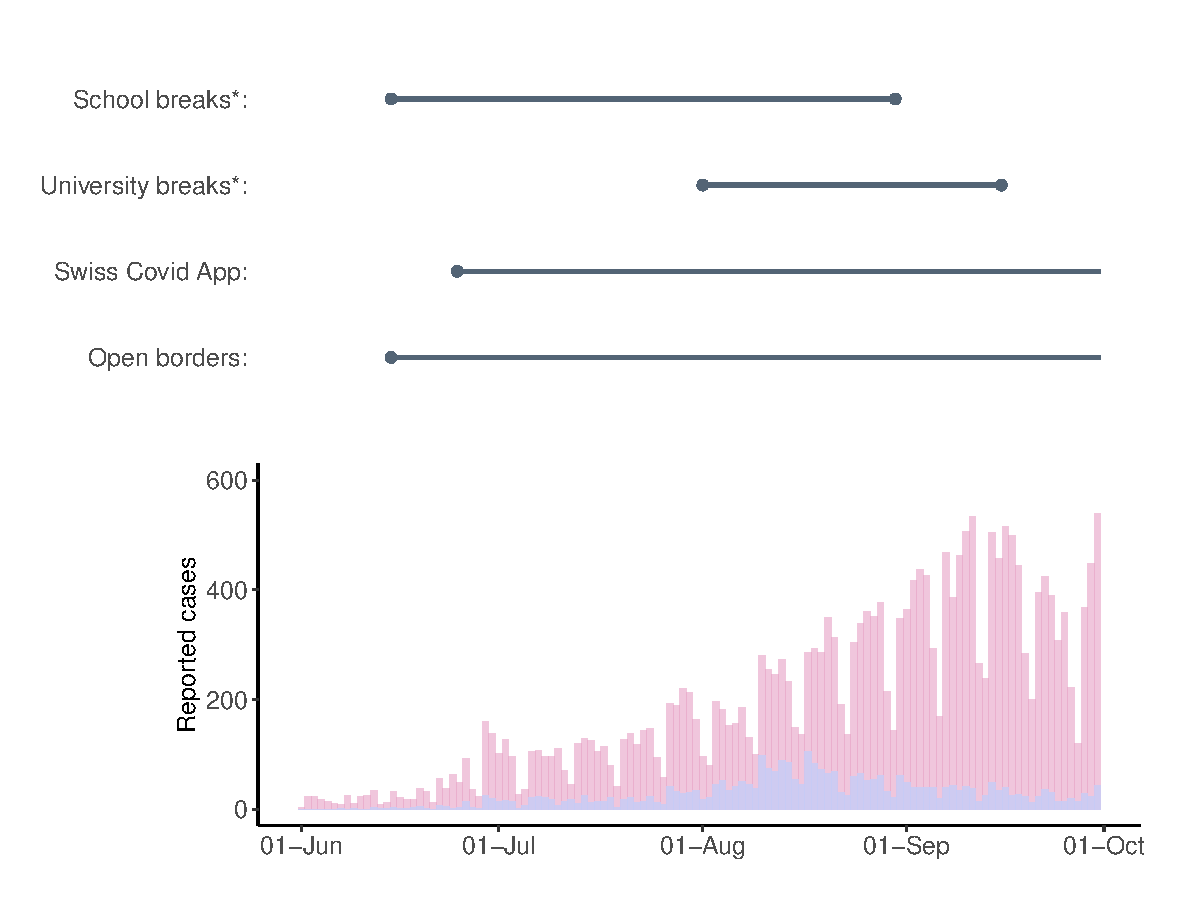
\includegraphics[scale=0.5]{regulation_cases_reported_2021-03-05.pdf}
\caption{Reported cases and major events: y-axis reported cases; x-axis time of interest; pink bars show all reported cases per day and violet bars show only cases with most likely place of infection abroad. *Official break of universities (might change for different subjects) and cantons have different school holiday, here we took earliest and latest holiday day. More details on quarantine measures  \href{https://www.fedlex.admin.ch/eli/cc/2021/61/de}{here}.}
\end{figure}
\begin{multicols}{2}

\end{multicols}
\begin{figure}[h]
\centering
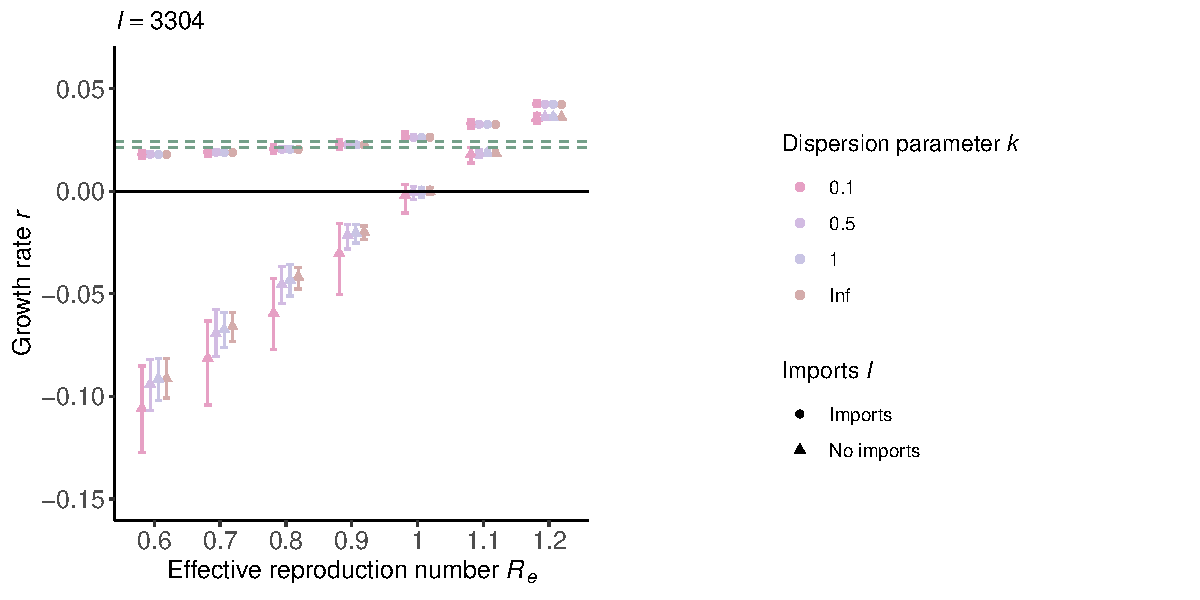
\includegraphics[scale=0.5]{growth_r_imports_infect_reported_2021-02-24.pdf}
\caption{Impact of imports on the epidemic growth rate: y-axis the epidemic growth rate; x-axis different $R_e$ values; intervals show the inter-quantile range (IQR). Abbreviations: k, dispersion parameter; I, number of imports.}
\end{figure}
\begin{multicols}{2}

\end{multicols}
\begin{figure}[h]
\centering
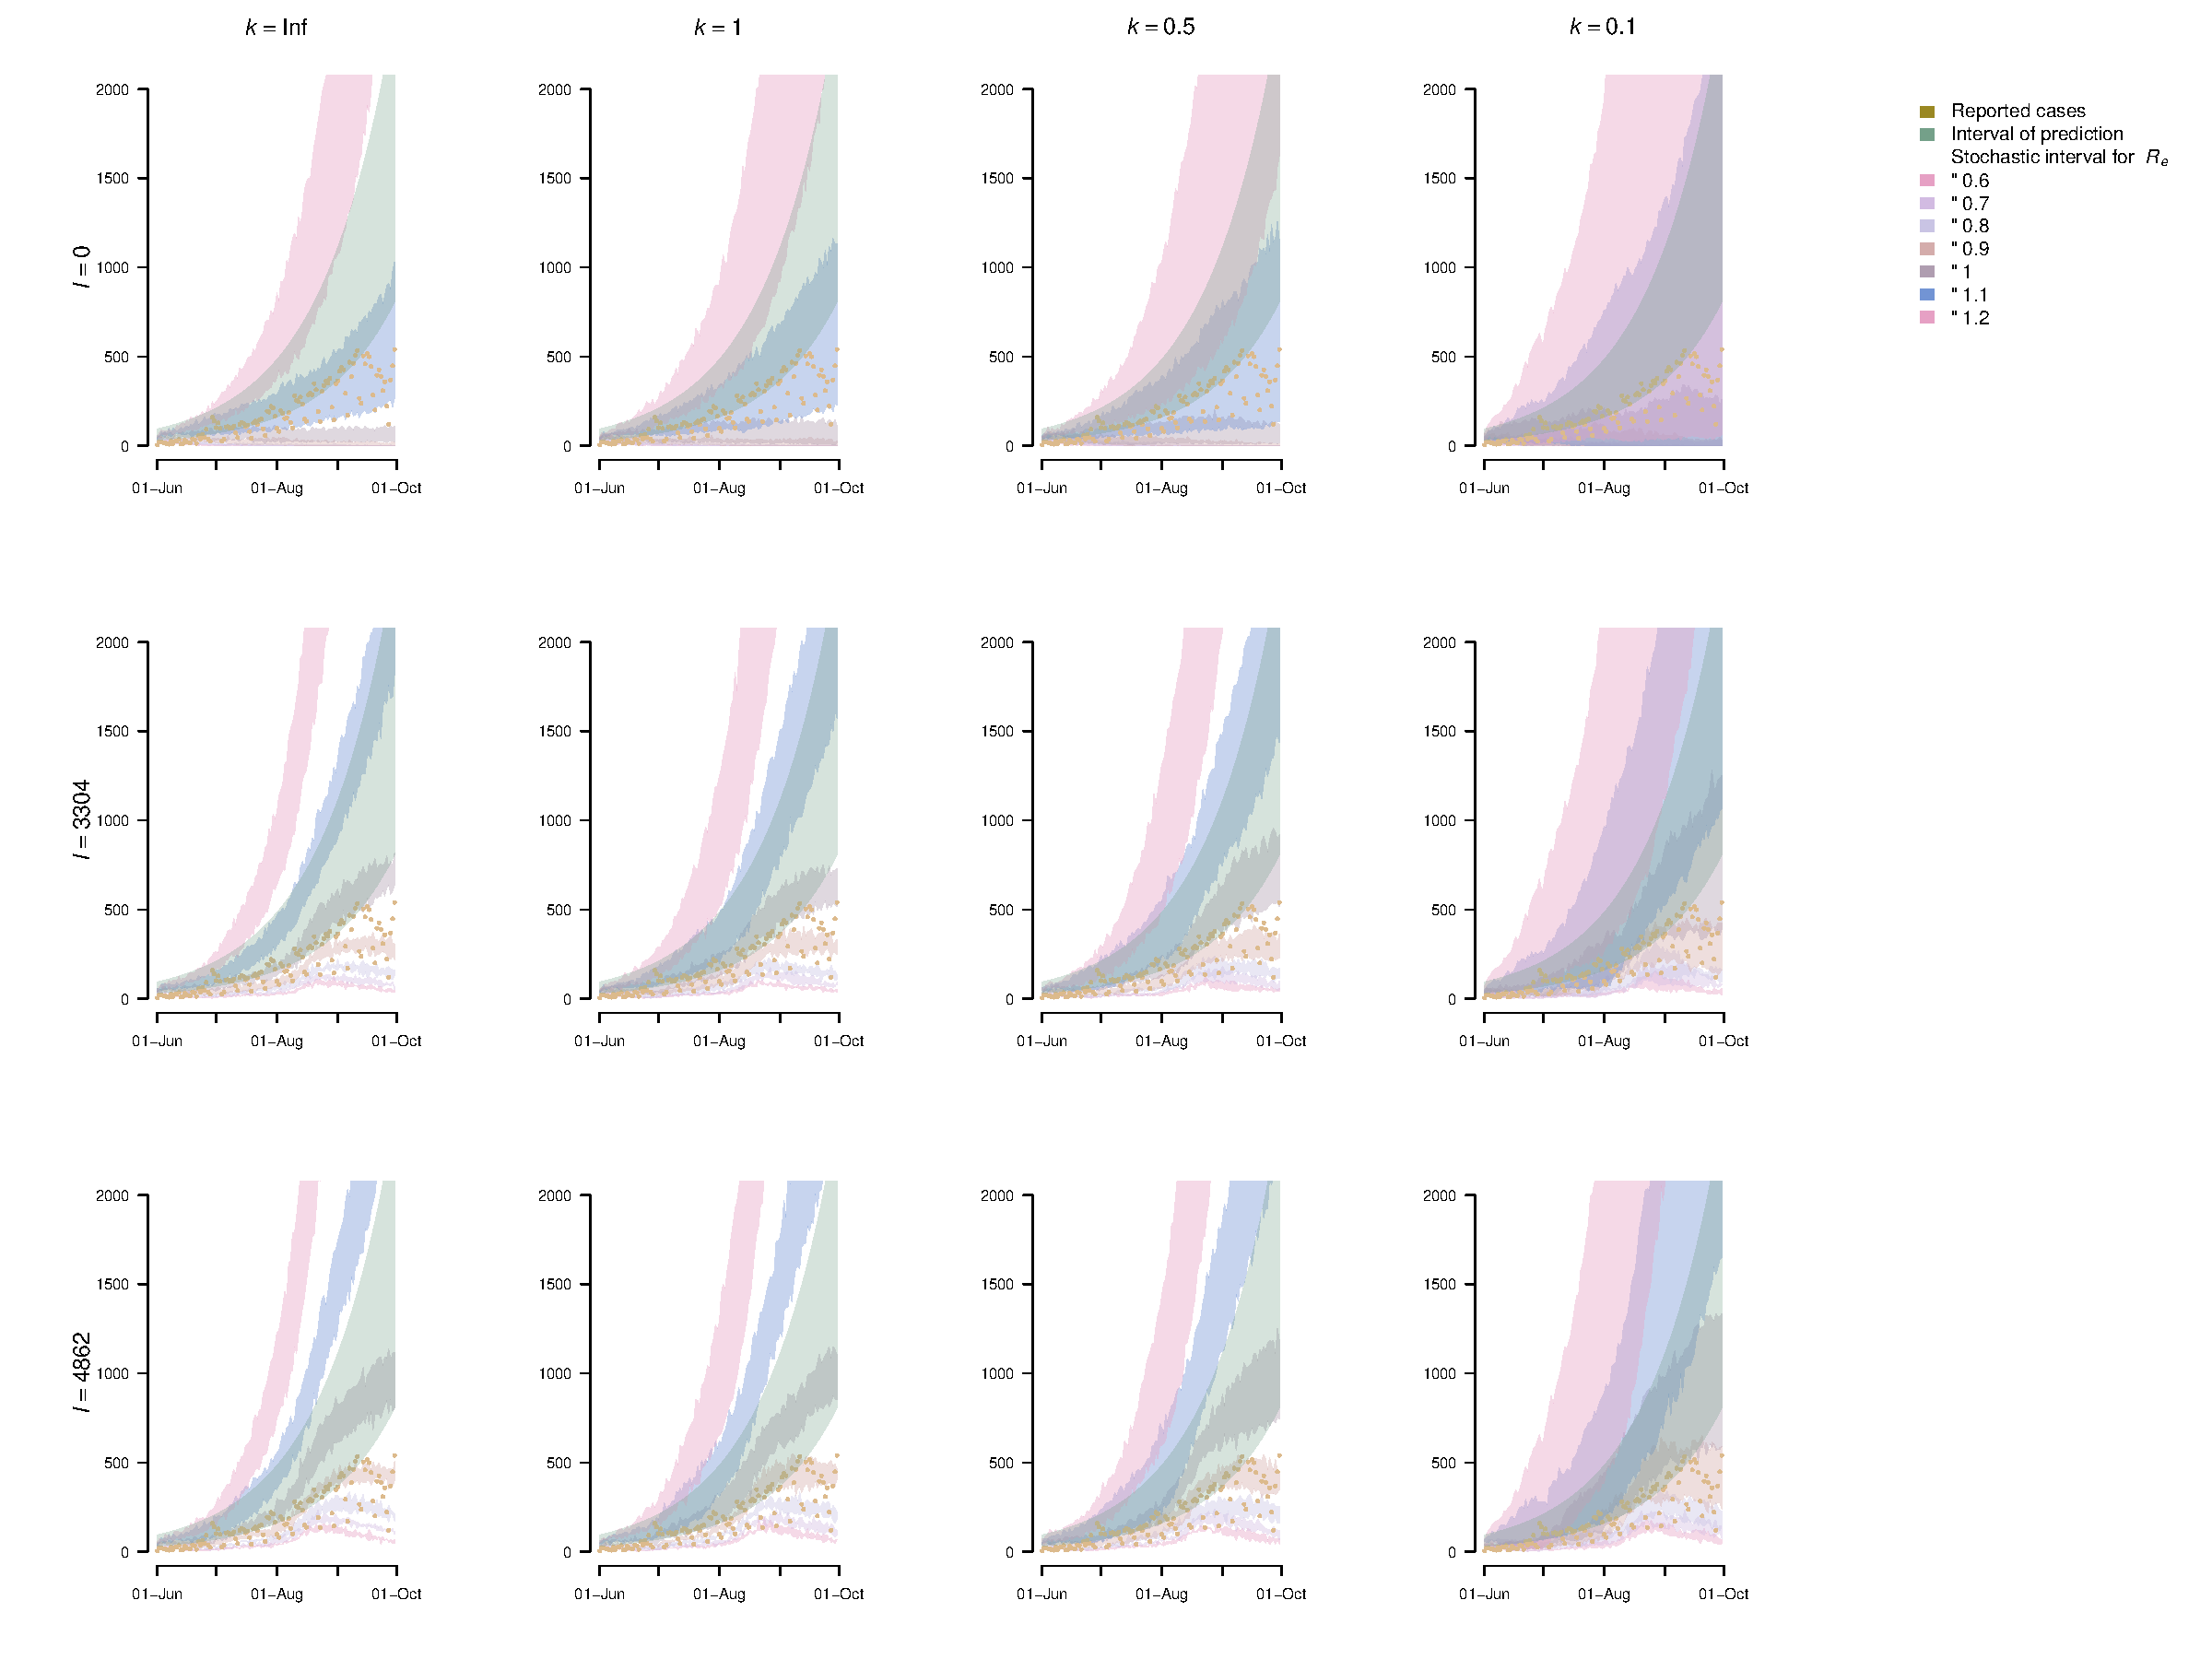
\includegraphics[scale=0.4]{sim3_cases_d_imports_infect_2021-02-24.pdf}
\caption{Impact of imports on the cases per day: y-axis cases per day; x-axis time of interest. Yellow dots show the reported cases per day and green area shows the predicted cases per day. Abbreviations: $k$, dispersion parameter; $I$, number of imports.}
\end{figure}

\begin{multicols}{2}

\section{Discussion}
The SARS-CoV-2 epidemic grew from a few dozen confirmed cases per day in early June 2020 to several hundred by the end of September 2020. 
Switzerland is a relatively small country with a few million inhabitants, but due to its location (and its wealth) there is a high potential for travel to have a huge impact on the epidemic.
Therefore, the intrinsic high probability of extinction - due to the small number of cases in early June - may have been offset by travel.
We estimated a $R_e$ slightly above 1 for the time of interest. So, the $R_e$ was around the critical value of 1, where small changes have a huge effect on the epidemic. 
Our stochastic simulations showed that the national epidemic had a $R_e$ below one, i.e. a value below the critical threshold. 
Travel-associated cases and their further transmission was a leading force that led to several hundred cases per day by the end of September 2020. 
Without any travel-associated cases, regardless of the dispersion parameter $k$, only an $R_e$ above 1 could explain the observed Swiss epidemic. 
In our analysis, we only accounted for travel-associated case that were successfully detected and thus stoped their transmission chain or for travel-associated case that infected further in the same way as cases that were infected in Switzerland.
\textcolor{red}{Need to include sth on age differences.}


\textcolor{red}{Nevertheless, our method has limitations that need to be addressed. We did not account for different behaviour in different groups. With our model we could only estimate a broad spectrum for the effect of travel-associated cases}

Quantifying the role of imports on the national dynamics of SARS-CoV-2 epidemics requires further investigation. 
In Switzerland, travel-associated case might have had a considerable impact on the national dynamics and could explain the growth of the SARS-CoV-2 epidemic during summer 2020. 
Our results underline the importance of improved surveillance for international travellers in order to better control the spread of SARS-CoV-2.

\section{Acknowledgement}
We thank the FOPH.

\section{Author contributions}
MLR, EBH, JR, and CLR conceived the study and contributed to the analysis of the results. 
MLR performed the analysis and wrote the first draft of the manuscript. 
%NH gave important inputs for the analysis and interpretation. 
All authors read and approved the final manuscript.

\section{Funding}
European Union’s Horizon 2020 research and innovation programme - project EpiPose (No 101003688). Swiss National Science Foundation (grant 196046)

\section{Reference}
\printbibliography[heading=none]

\end{multicols}

\clearpage
\section{Supplementary}
\begin{suppfigure}[h]
\centering
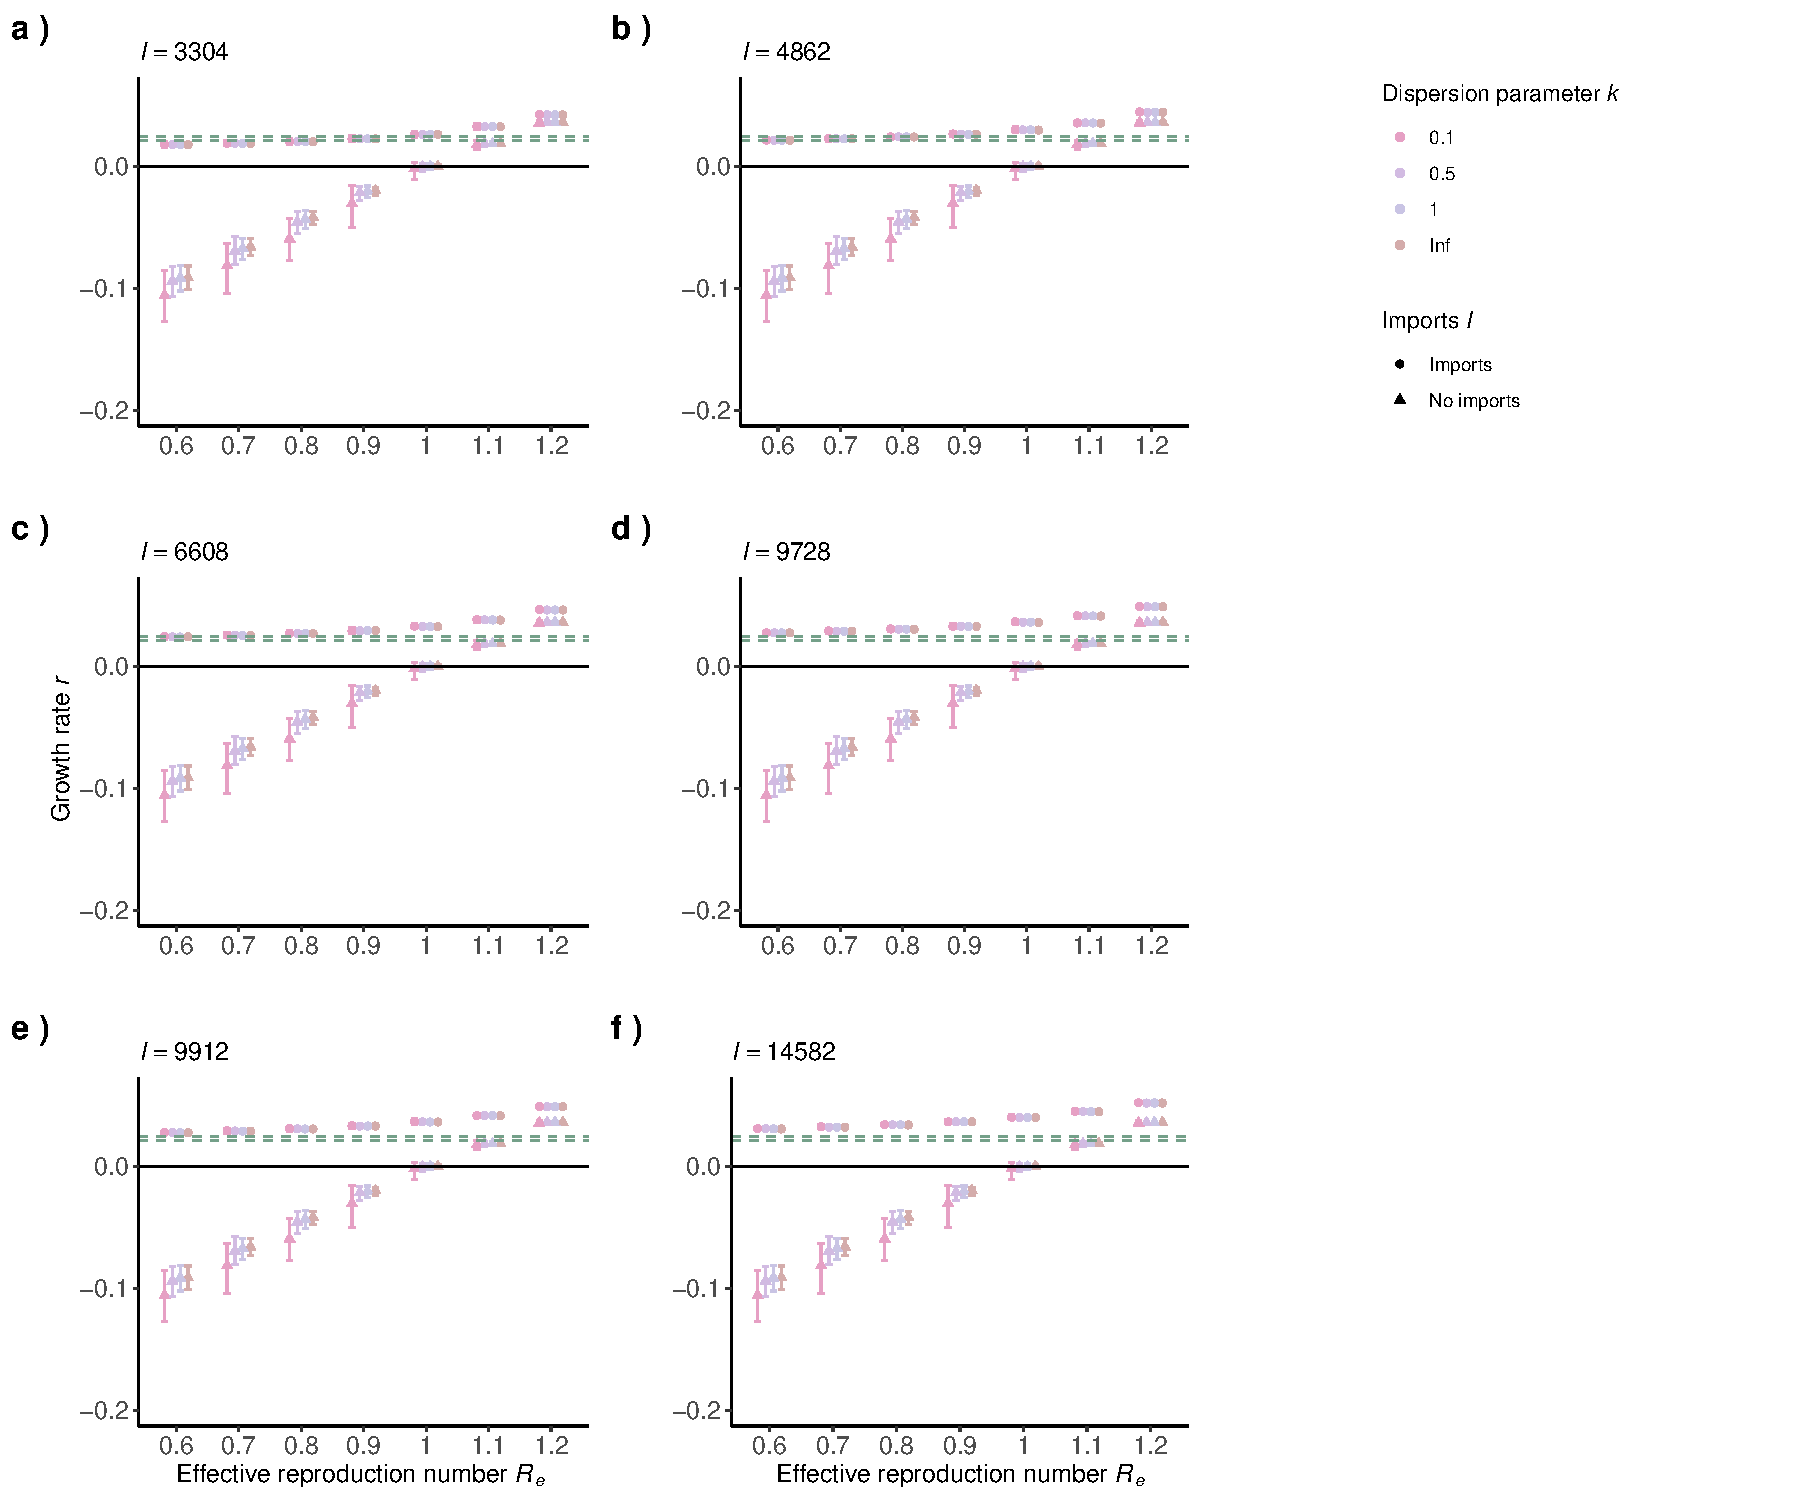
\includegraphics[scale=0.5]{growth_r_imports_infect_2021-02-24.pdf}
\caption{Impact of travel-associated cases \emph{I} that infect further on the epidemic growth rate: y-axis the epidemic growth rate; x-axis different $R_e$ values; intervals show the inter-quantile range (IQR). a) reported travel-associated cases. b) reported imports multiplied by following $1+ \frac{\Sigma ~of ~cases ~with ~unknown ~origin }{\Sigma ~of ~all ~confirmed ~cases}$. c) $a)$ multiplied with 2. d) $b)$ multiplied with 2. e,f) $a)$ and $b)$ multiplied with 3, respectively. Abbreviations: k, dispersion parameter; I, number of travel associated cases.}
\end{suppfigure}
\clearpage
\begin{suppfigure}[h]
\centering
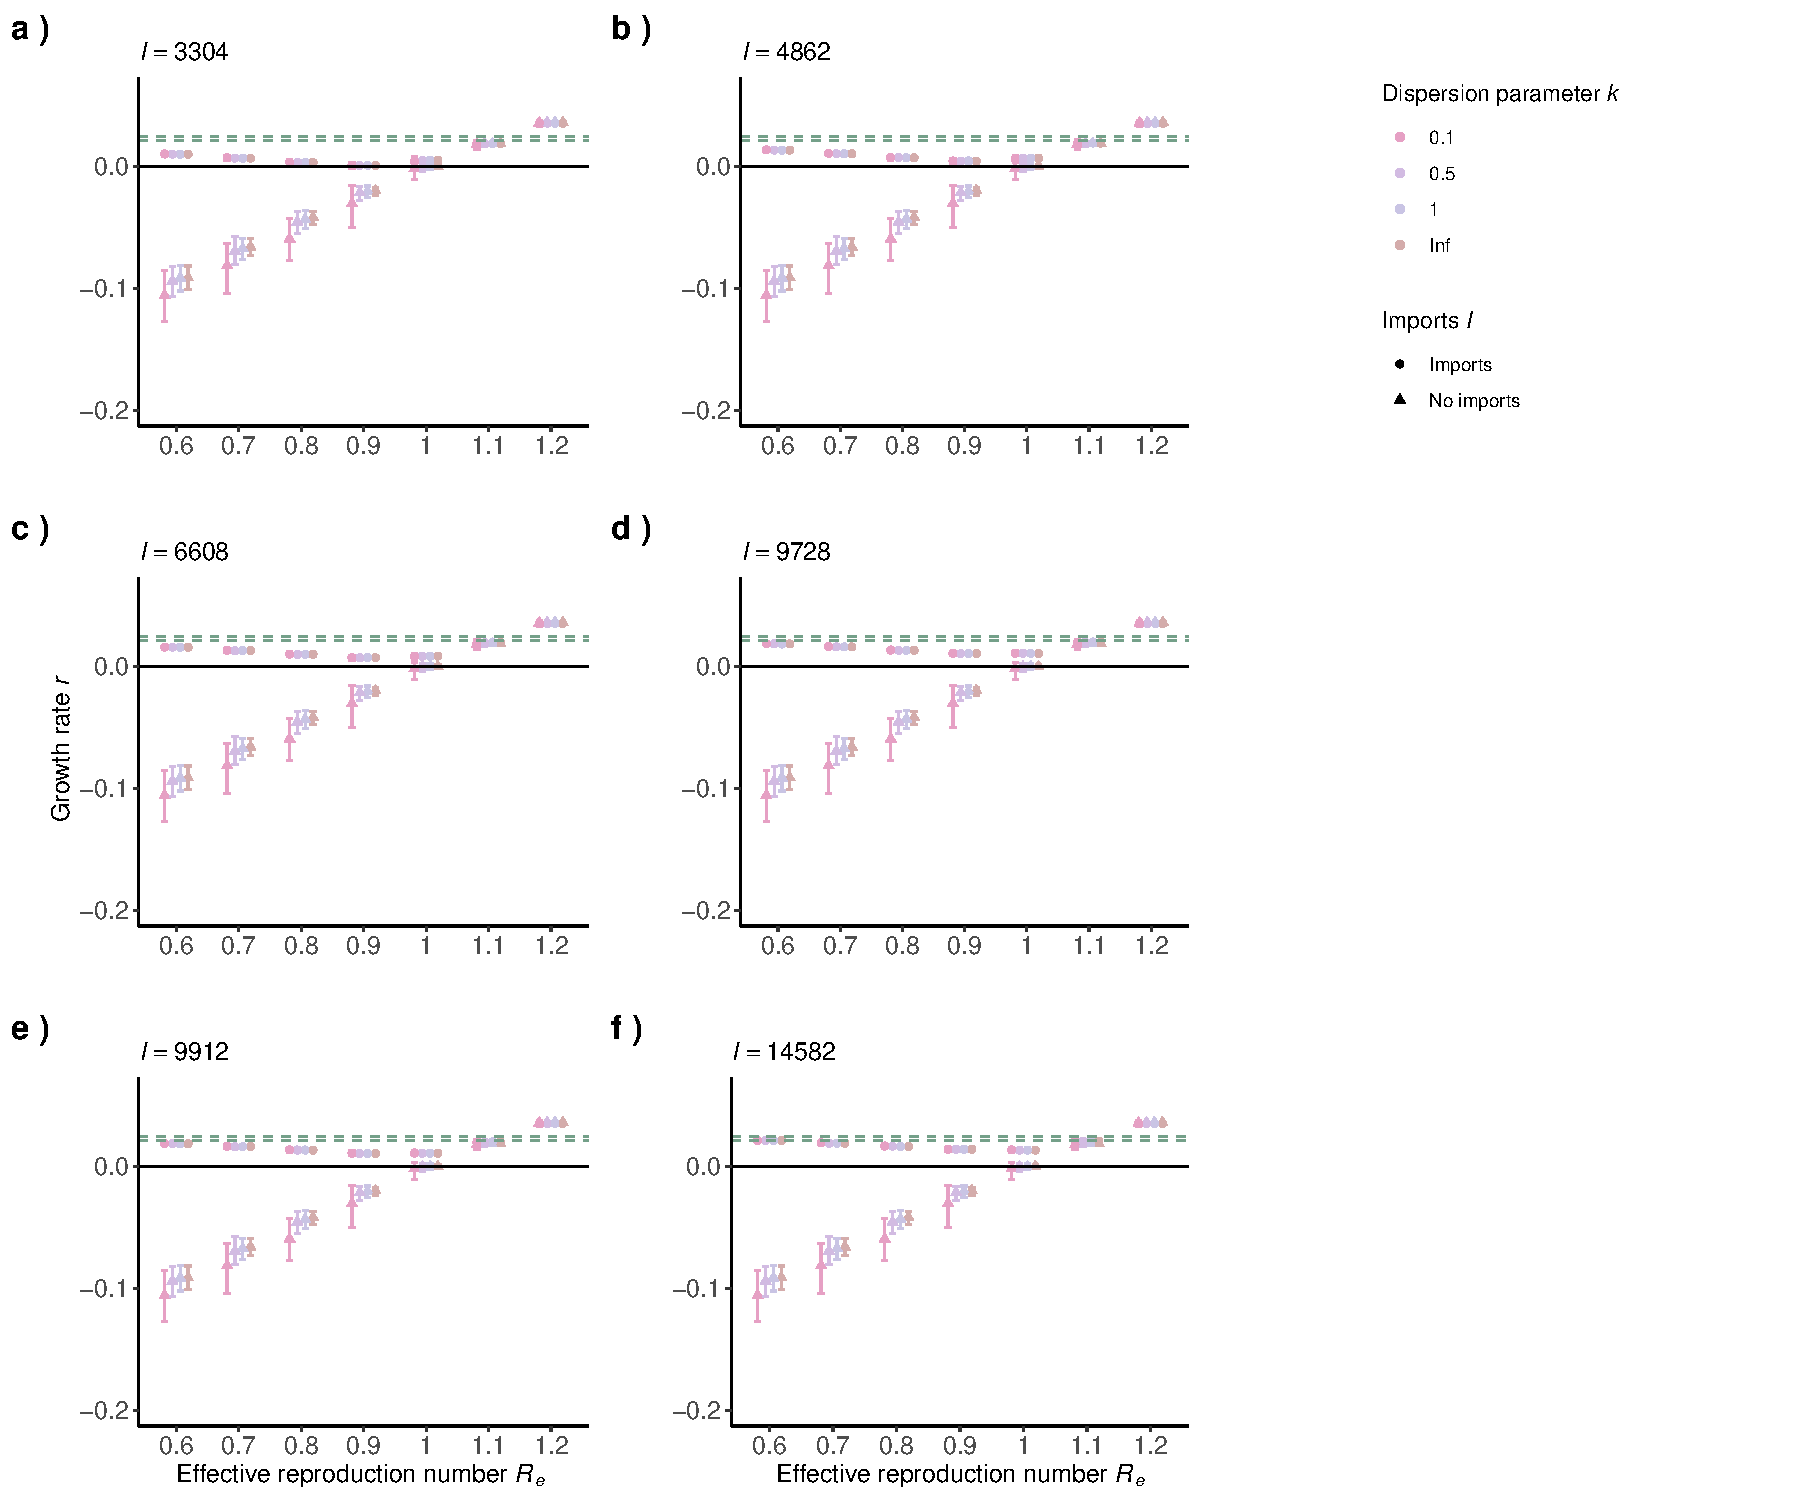
\includegraphics[scale=0.5]{growth_r_imports_2021-02-24.pdf}
\caption{Impact of travel associated cases \emph{I} that do not infect further on the epidemic growth rate: y-axis shows the epidemic growth rate; x-axis different $R_e$ values; intervals show the inter-quantile range (IQR). a) reported travel associated cases. b) reported imports multiplied by following $1+ \frac{\Sigma ~of ~cases ~with ~unknown ~origin }{\Sigma ~of ~all ~confirmed ~cases}$. c) $a)$ multiplied with 2. d) $b)$ multiplied with 2. e,f) $a)$ and $b)$ multiplied with 3, respectively. Abbreviations: k, dispersion parameter; I, number of travel associated cases.}
\end{suppfigure}
\clearpage
\begin{suppfigure}[h]
\centering
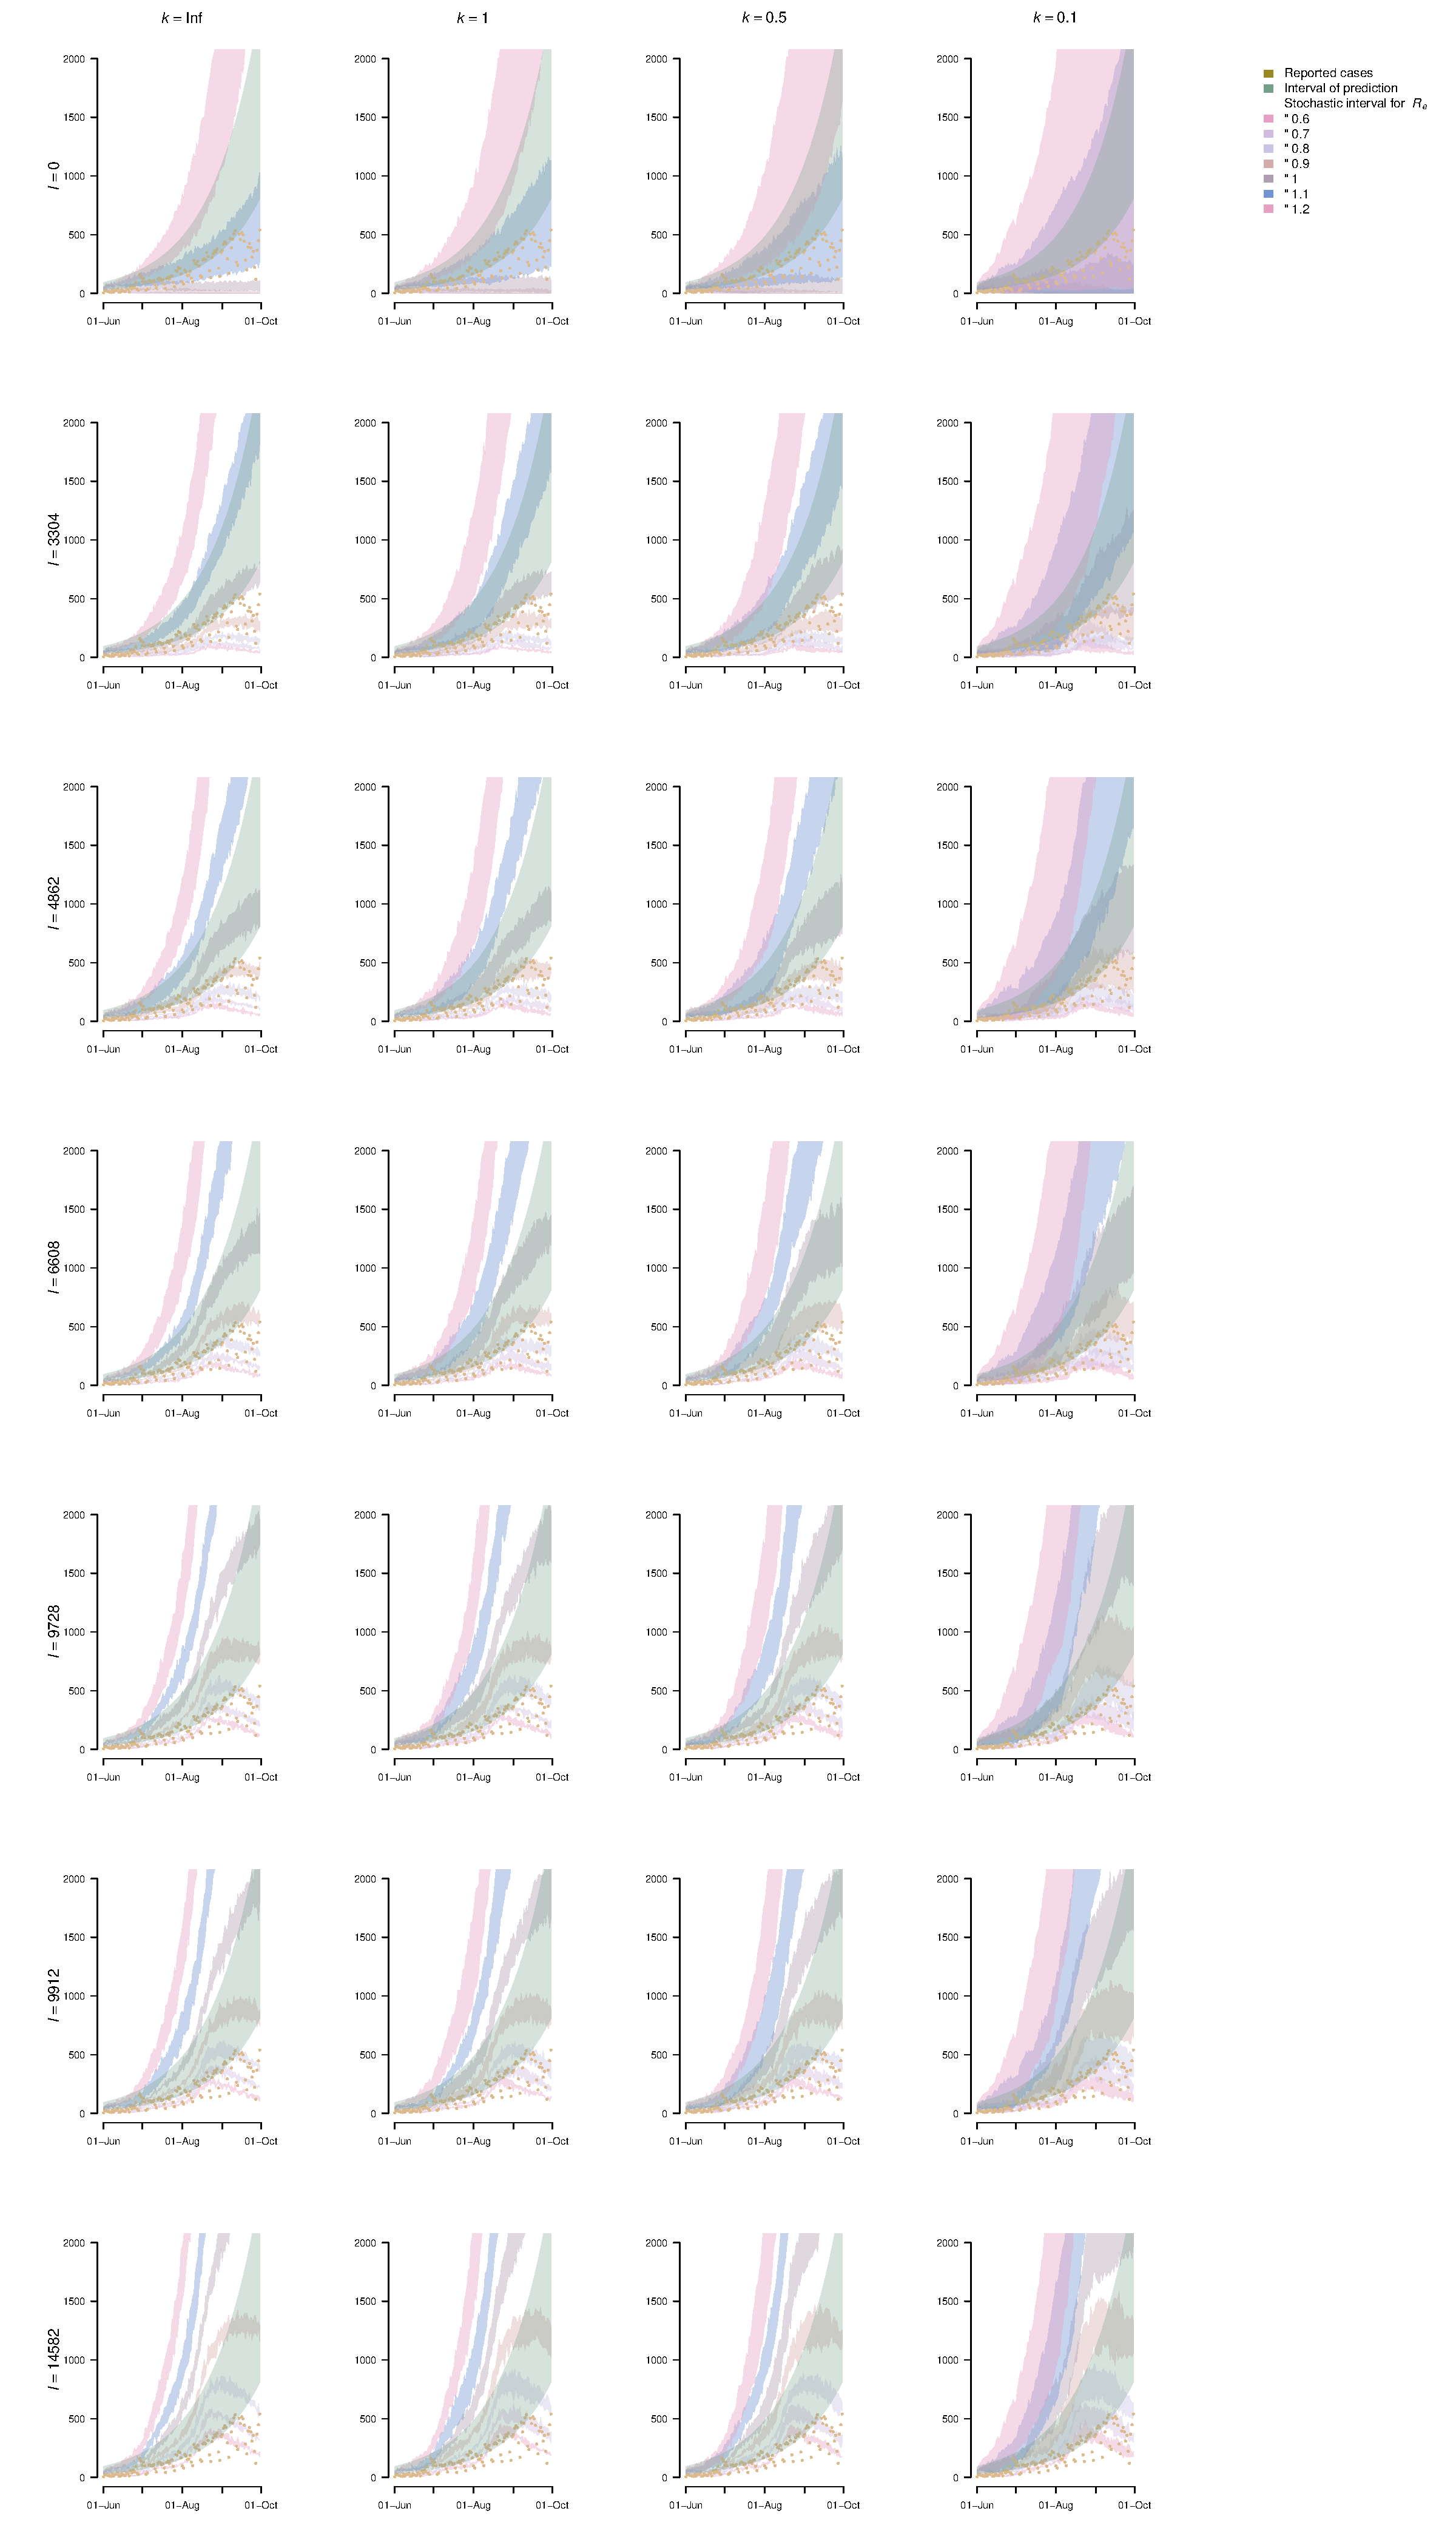
\includegraphics[scale=0.3]{sim_cases_d_imports_infect_2021-02-24.pdf}
\caption{Impact of travel-associated cases on the cases per day that infected further: y-axis cases per day; x-axis the time of interest. Different number of travel-associated cases \emph{I} were added to a stochastic branching model whereby these \emph{I} could transmit further: \emph{I} was zero, reported \emph{I}, reported \emph{I} multiplied by $1+ \frac{\Sigma ~of ~cases ~with ~unknown ~origin }{\Sigma ~of ~all ~confirmed ~cases}$, and these multiplied with 2 and 3, respectively. Yellow dots show the reported cases per day and green area shows the predicted cases per day. Abbreviations: k, dispersion parameter; I, number of travel associated cases.}
\end{suppfigure}
\clearpage
\begin{suppfigure}[h]
\centering
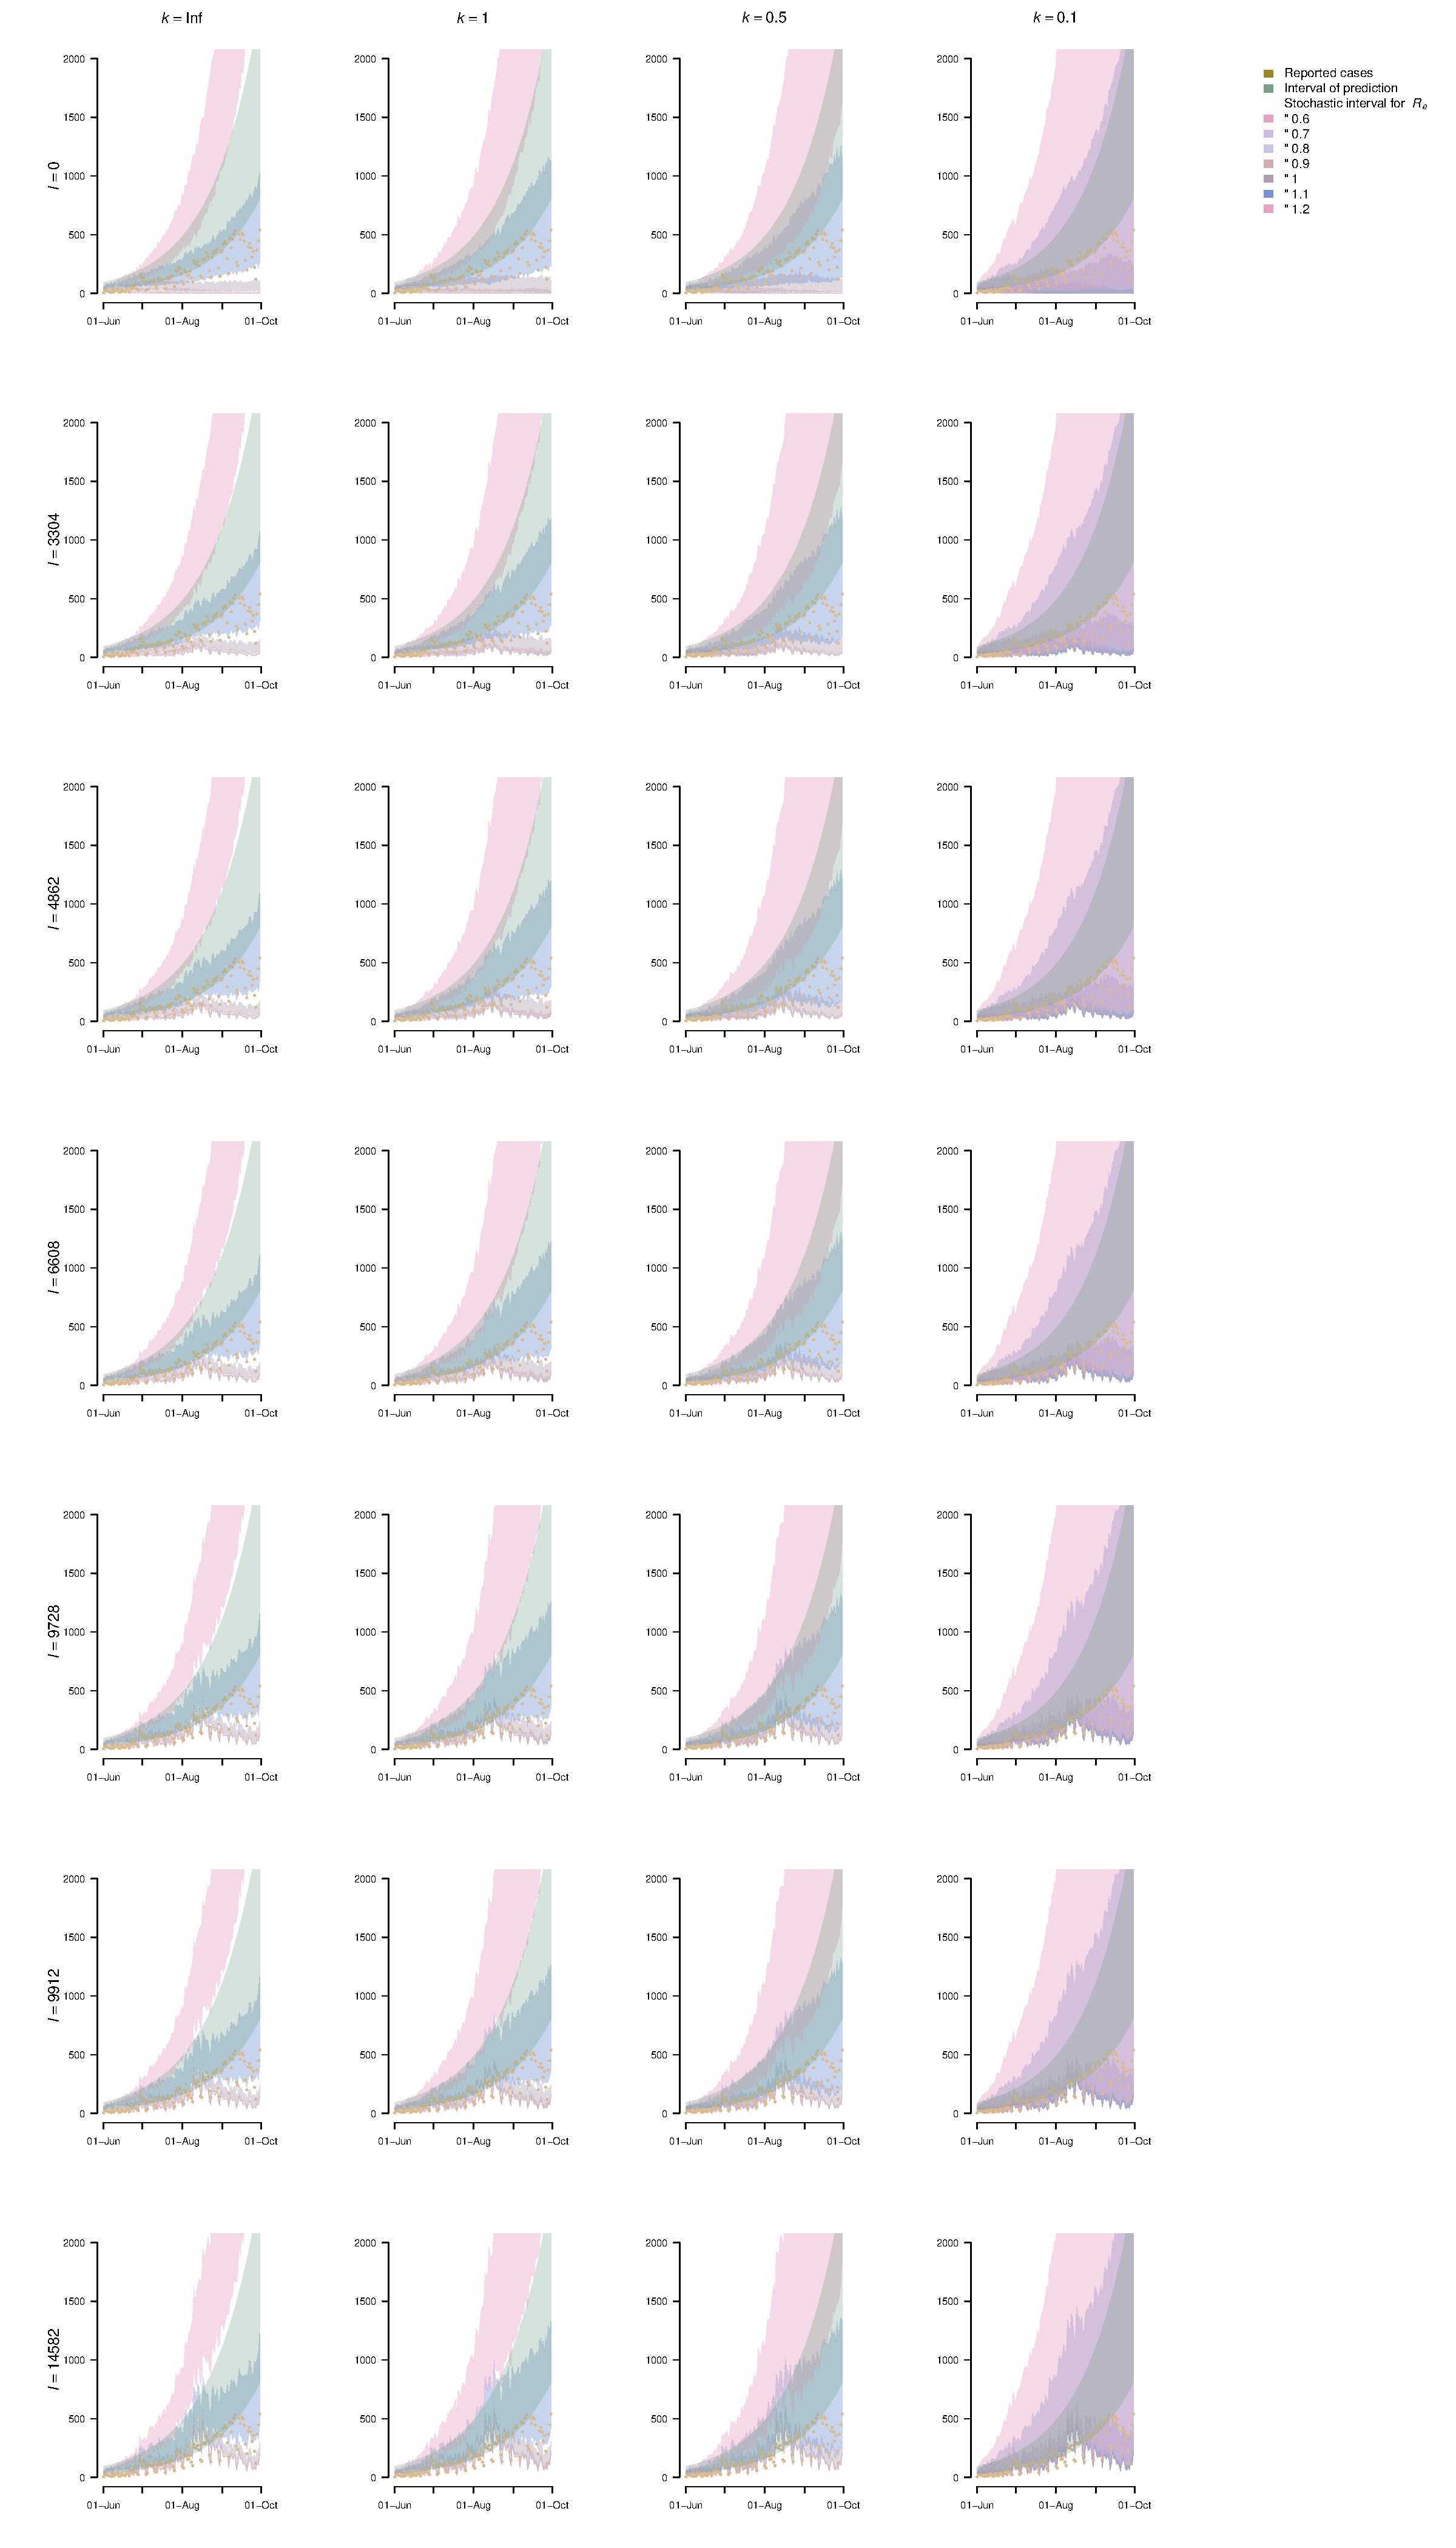
\includegraphics[scale=0.3]{sim_cases_d_imports_2021-02-24.pdf}
\caption{Impact of travel-associated cases on the cases per day that did not infect further: y-axis cases per day; x-axis the time of interest. Different number of travel-associated cases \emph{I} were added to a stochastic branching model whereby these \emph{I} could transmit further: \emph{I} was zero, reported \emph{I}, reported \emph{I} multiplied by $1+ \frac{\Sigma ~of ~cases ~with ~unknown ~origin }{\Sigma ~of ~all ~confirmed ~cases}$, and these multiplied with 2 and 3, respectively. Yellow dots show the reported cases per day and green area shows the predicted cases per day. Abbreviations: k, dispersion parameter; I, number of travel associated cases.}
\end{suppfigure}
\clearpage
\begin{suppfigure}[h]
\centering
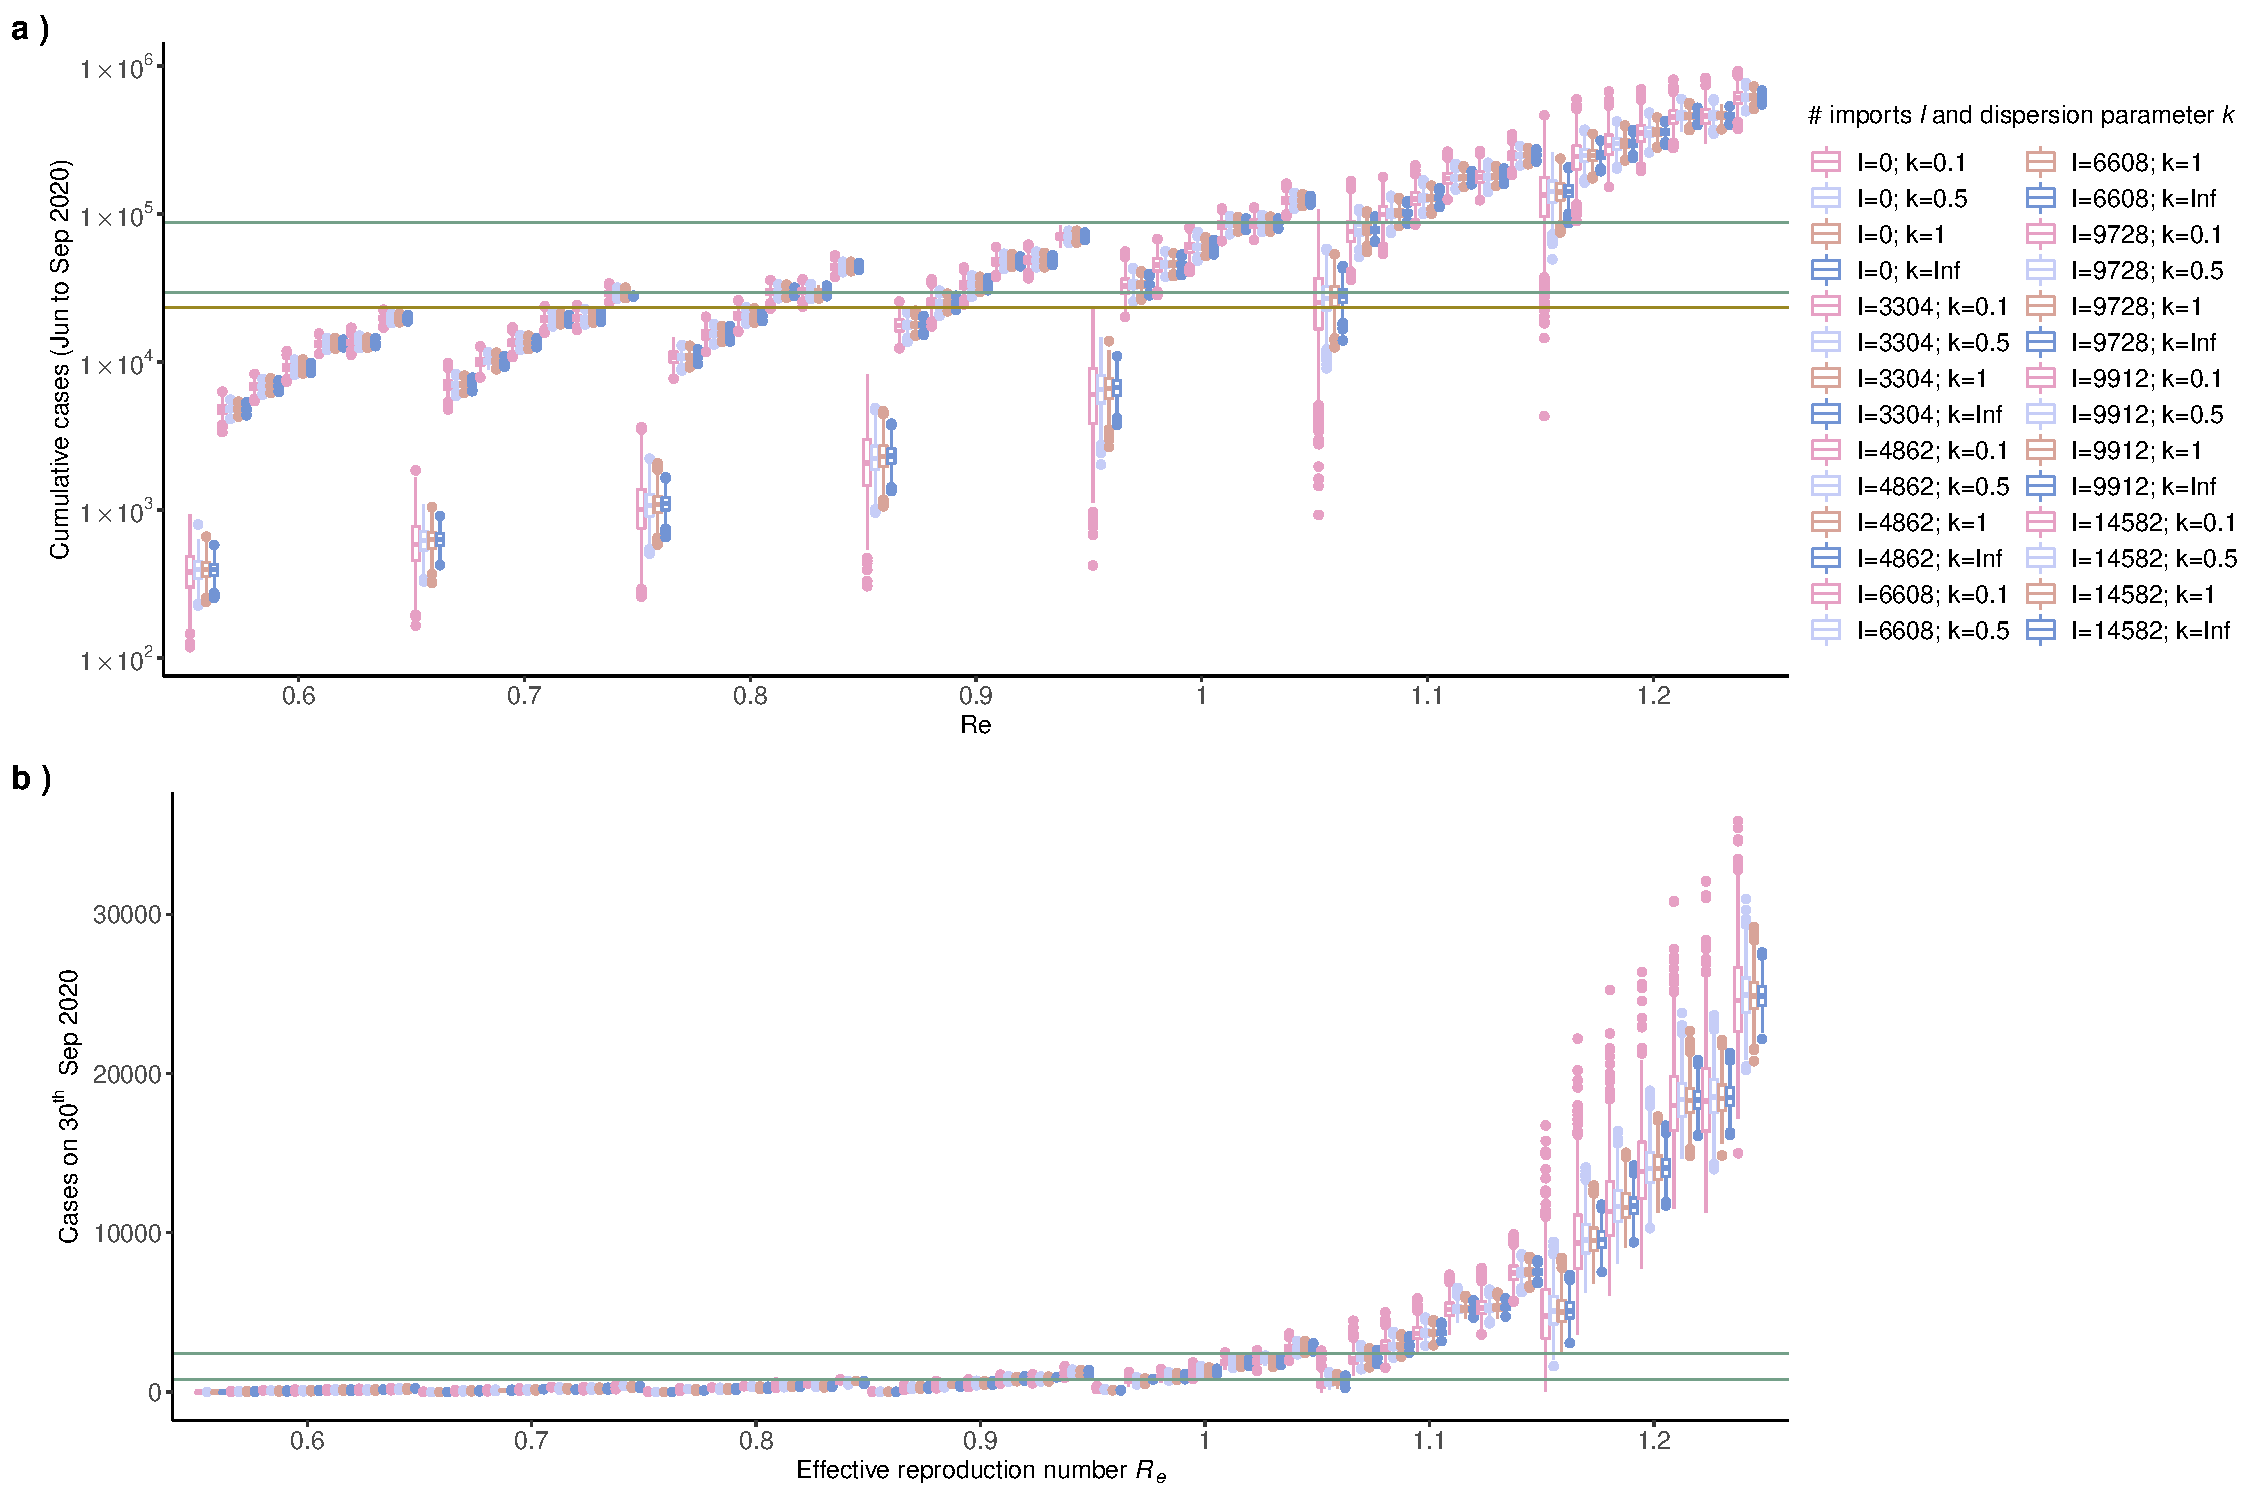
\includegraphics[scale=0.4]{size_scenarios_imports_infect_2021-02-24.pdf}
\caption{Cumulative cases and final number of cases regarding the different scenarios whereby travel-associated cases infected further.Yellow line shows the reported cases during $1^{st}$ of June to $30^{th}$ of September 2020. The area between the green lines shows the predicted cases during $1^{st}$ of June to $30^{th}$ of September 2020 and on the $30^{th}$ of September 2020. Abbreviations: k, dispersion parameter; I, number of travel associated cases.}
\end{suppfigure}
\clearpage
\begin{suppfigure}[h]
\centering
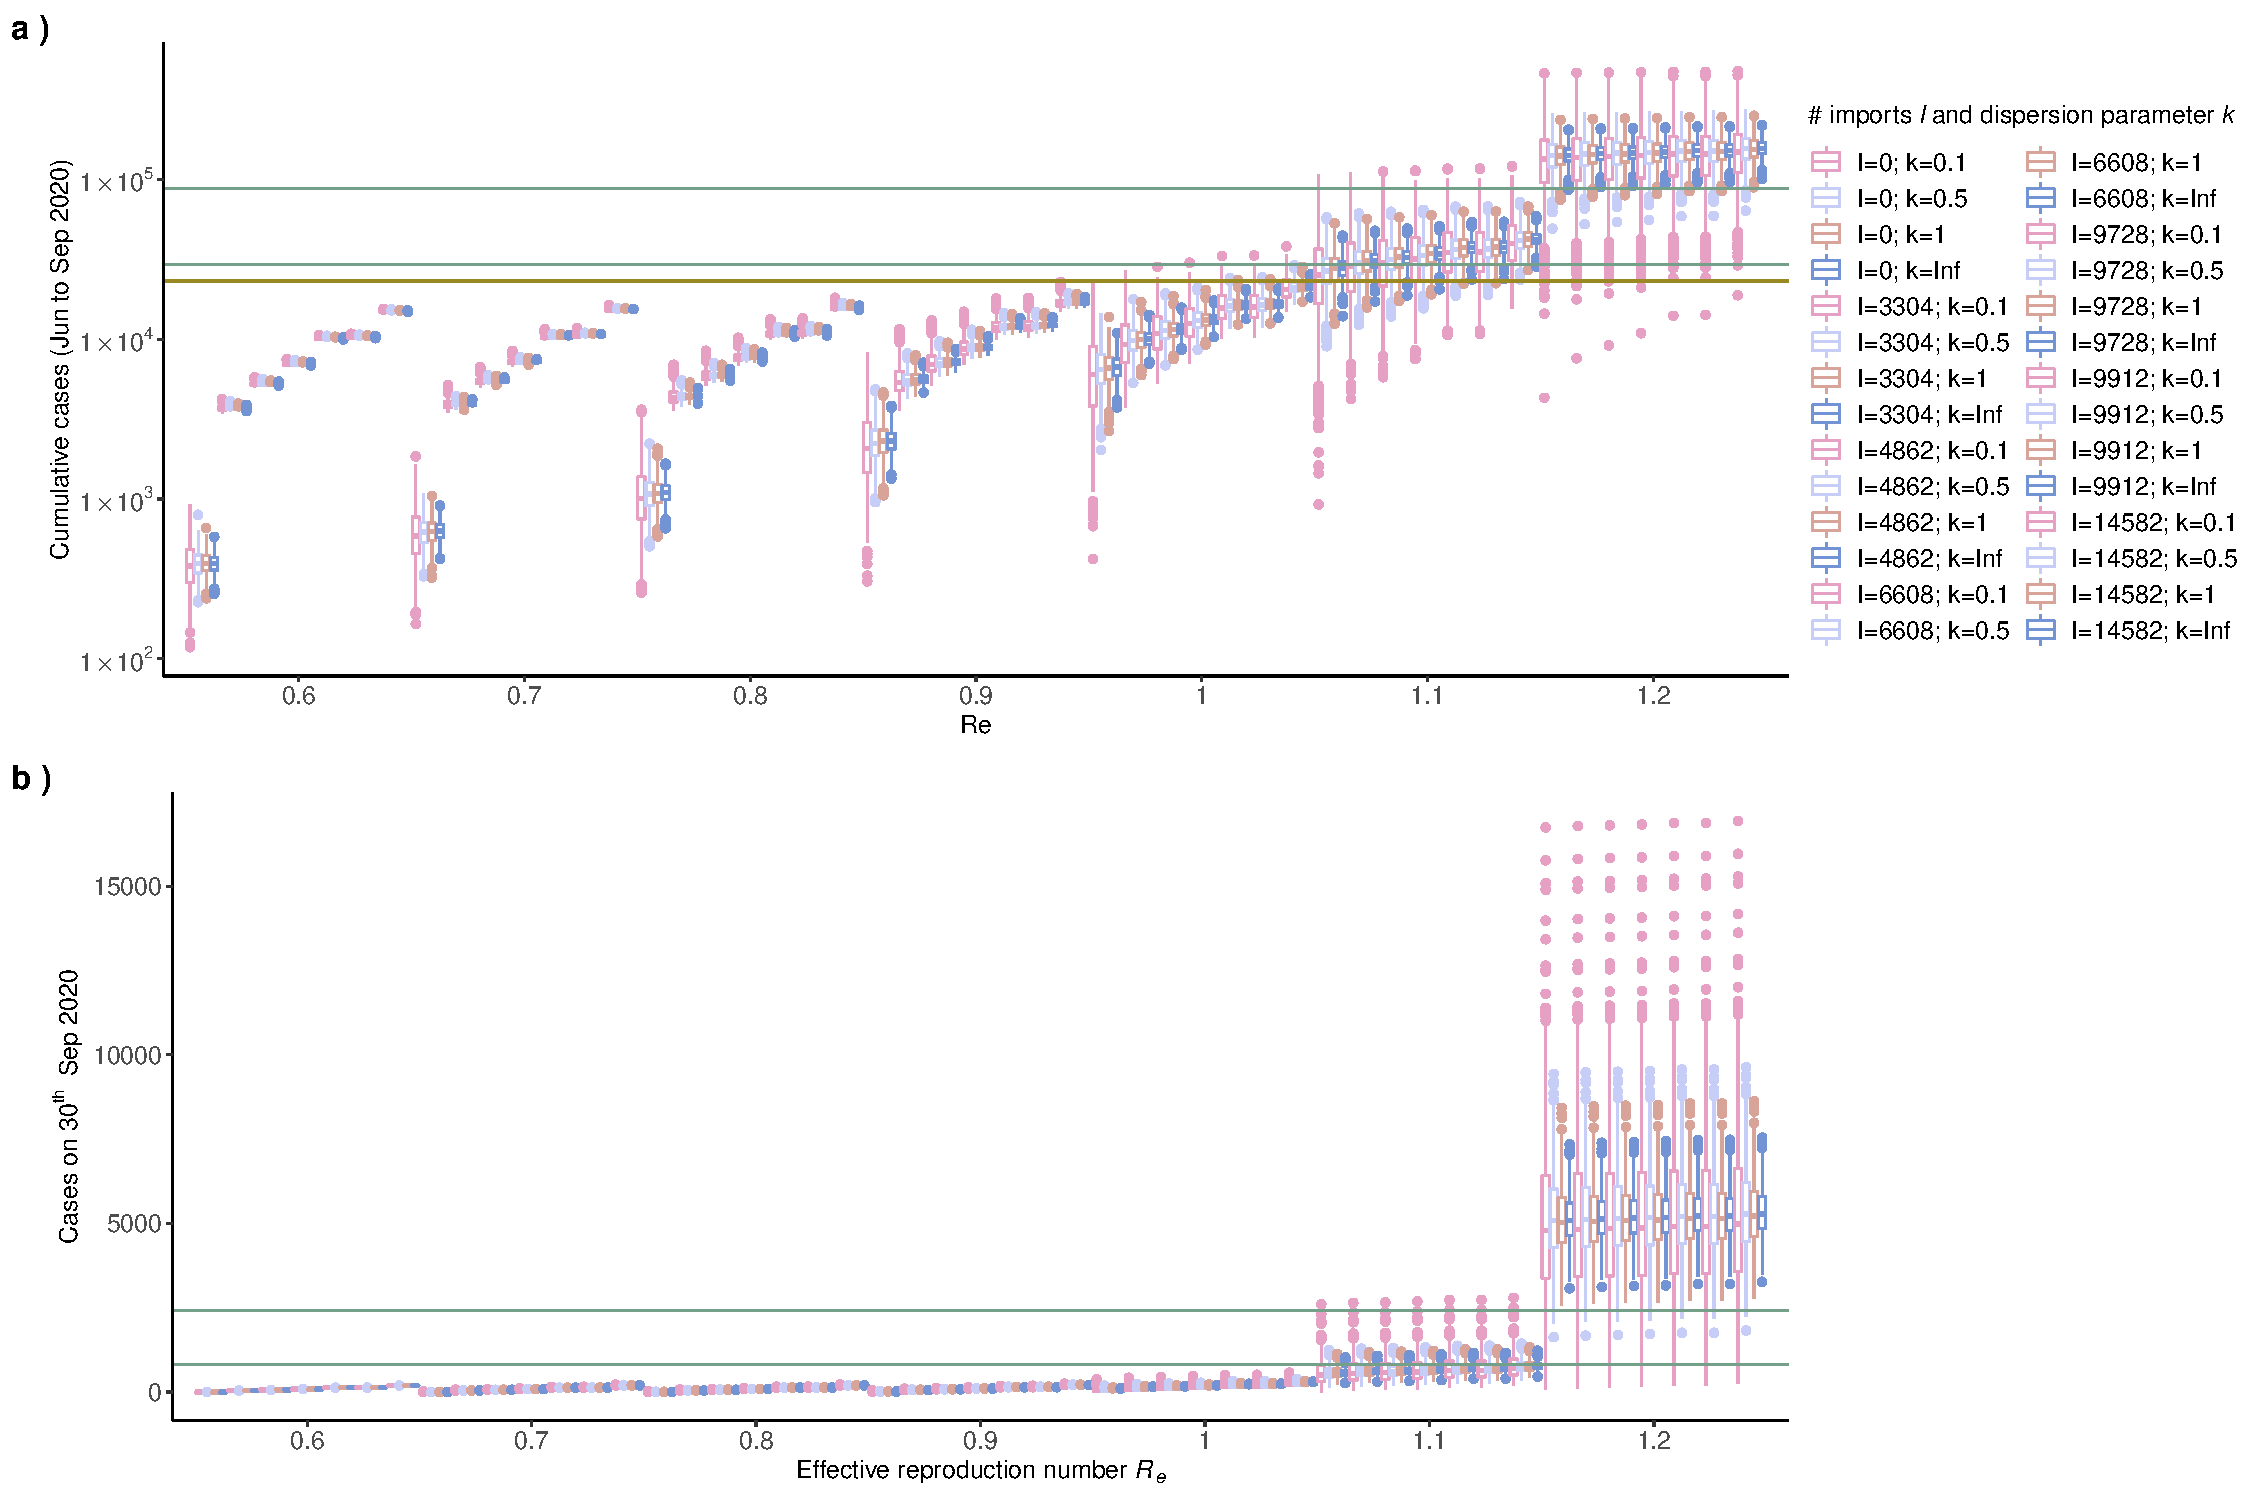
\includegraphics[scale=0.4]{size_scenarios_imports_2021-02-24.pdf}
\caption{Cumulative cases and final number of cases regarding the different scenarios whereby travel-associated cases did not infect further. Yellow line shows the reported cases during $1^{st}$ of June to $30^{th}$ of September 2020. The area between the green lines shows the predicted cases during $1^{st}$ of June to $30^{th}$ of September 2020 and on the $30^{th}$ of September 2020. Abbreviations: k, dispersion parameter; I, number of travel associated cases.}
\end{suppfigure}
\clearpage
\begin{suppfigure}[h]
\centering
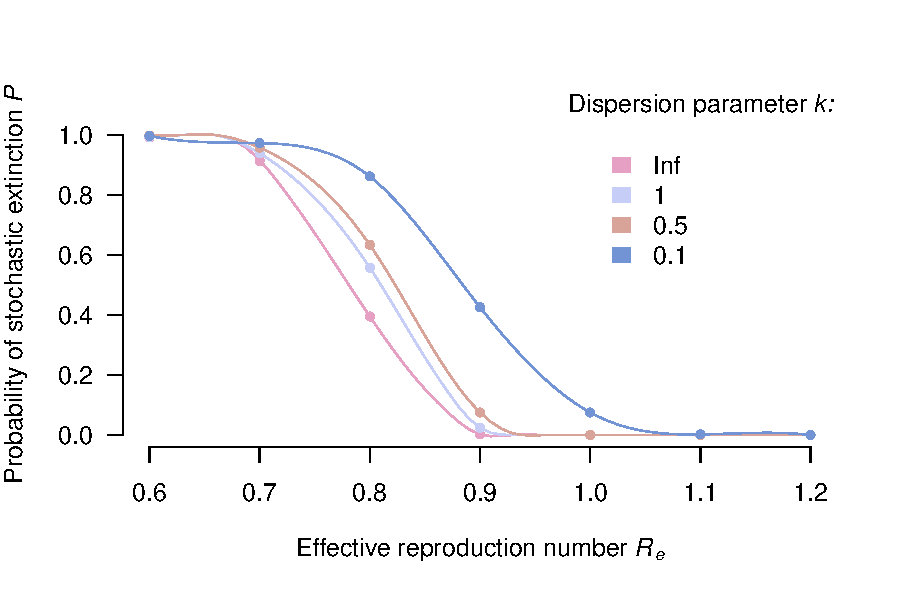
\includegraphics[scale=0.5]{P_extinction_2021-02-26.pdf}
\caption{Probability of stochastic extinction when 50 cases for each of the previous five days before the simulation started were used as seeds.}
\end{suppfigure}
\clearpage
\begin{suppfigure}[h]
\centering
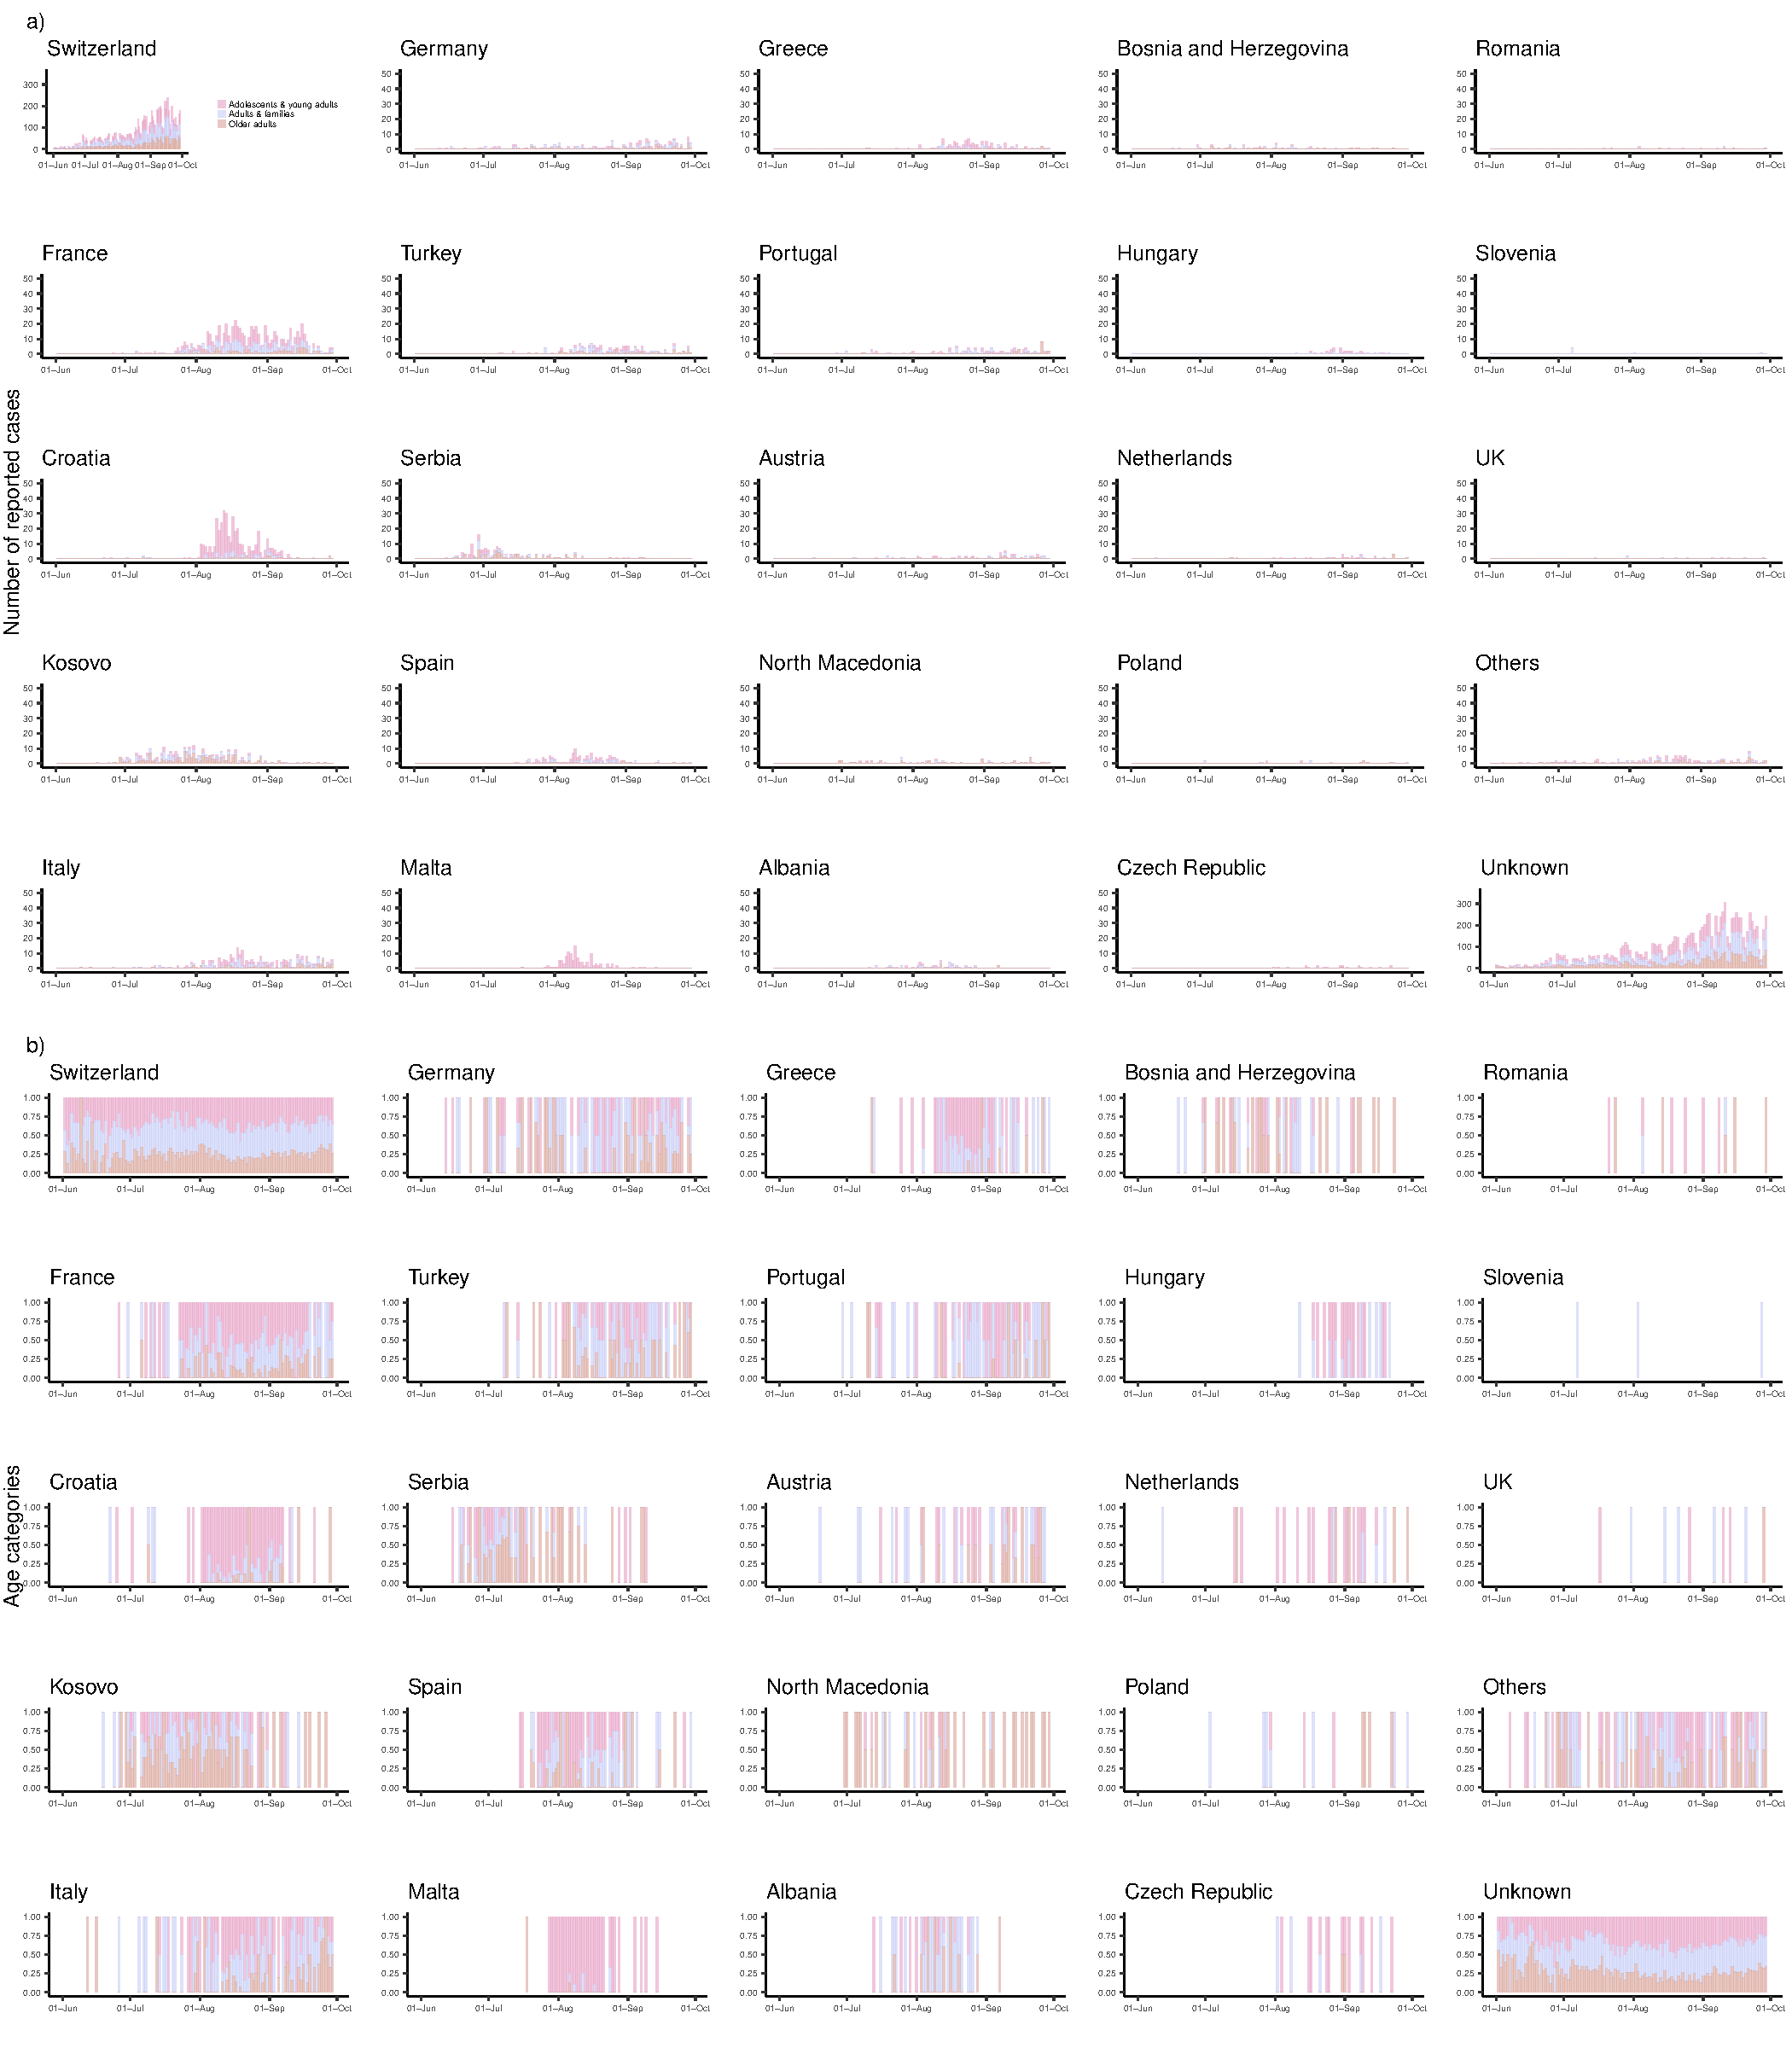
\includegraphics[scale=0.4]{imports_per_country_day_2021-03-05.pdf}
\caption{Reported cases and the most likely place of infection. a) y-axis and x-axis shows time of interest and number of reported cases b) y-axis and x-axis shows time of interest and proportion cases by different categories, i.e., adolescents and young adults (16-30 years), adults and families (31-50 and children up to 15 years), and older adults ($>$50 years).}
\end{suppfigure}
\clearpage
\begin{suppfigure}[h]
\centering
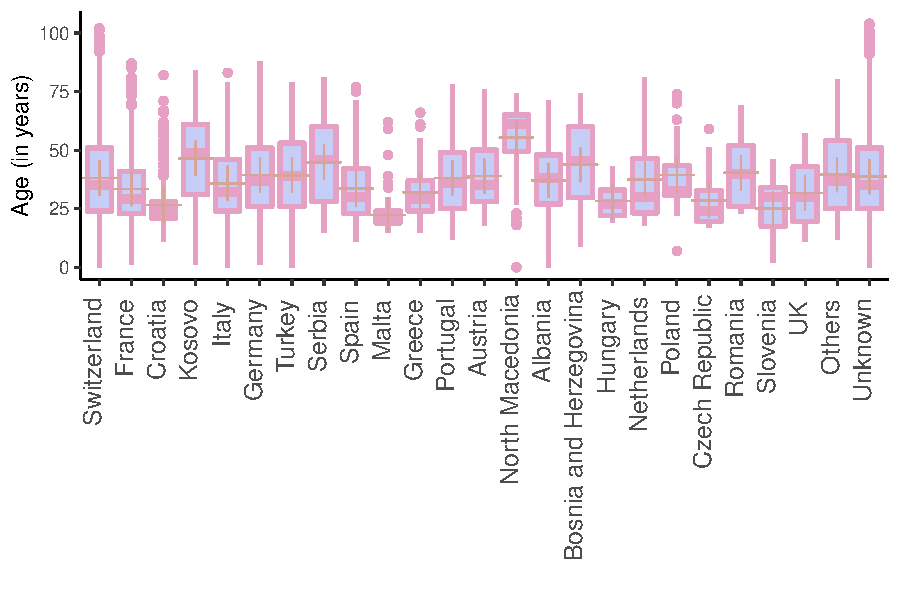
\includegraphics[scale=0.4]{age_percountry_2021-03-05.pdf}
\caption{Age distribution for reported cases by the most likely place of infection. y-axis and x-axis shows age and most likely infection place; + represents the mean.}
\end{suppfigure}

\end{document}
